\chapter{Syntax-driven design of neural-specific enhancers \textit{in vivo}}
\label{chap:chapter 2}

%%%%%%%%%%%%%%%%%%%%%%%%%%%%%%%%%%%%%%%%%%%%%%%%%%%%%%%%%%%%%%%%%%%%%%%%%%%%%%%%
\section{Abstract}
%%%%%%%%%%%%%%%%%%%%%%%%%%%%%%%%%%%%%%%%%%%%%%%%%%%%%%%%%%%%%%%%%%%%%%%%%%%%%%%%

The syntax of an enhancer consists of the organization of the transcription factor binding sites (TFBSs) it contains. To explore how the activity and specificity of an enhancer is encoded by syntax, we constructed a synthetic library in which all 460,800 sequences share the same five TFBSs but vary in their arrangement. Only a fraction of these organizations are active enhancers, demonstrating that syntax can be a major driver of enhancer function. From this data, we trained deep learning models to predict enhancer activity and found that enhancer function is readily predictable from syntax alone, and that predictions are largely driven by the additive combination of 2-site and 3-site combinations. Guided by the syntax model, we designed 192 synthetic enhancers with predicted tissue-specificity. 93\% (179/192) of our designs tuned activity in the intended direction, and 46\% (89/192) exhibited the desired tissue-specific activity. Our results demonstrate that syntax-based modeling provides a powerful and interpretable framework for understanding and engineering enhancer function.

%%%%%%%%%%%%%%%%%%%%%%%%%%%%%%%%%%%%%%%%%%%%%%%%%%%%%%%%%%%%%%%%%%%%%%%%%%%%%%%%
\section{Introduction}
%%%%%%%%%%%%%%%%%%%%%%%%%%%%%%%%%%%%%%%%%%%%%%%%%%%%%%%%%%%%%%%%%%%%%%%%%%%%%%%%

Enhancers are DNA sequences that control when and where genes are expressed. They function as genetic switches that activate transcription of nearby genes when bound by transcription factor (TF) proteins, often in specific developmental stages or cell types \cite{Levine2010-ry}. Short sequence motifs called transcription factor binding sites (TFBS) drive enhancer activity \cite{Stormo2010-xm}, and many enhancers obey certain organizational rules for these TFBSs, or “grammars” \cite{Jindal2021-zk}, that go beyond their mere presence. In this view, an enhancer’s function is not only controlled by the number, type, and affinity of the TFBSs it contains (the composition), but also by the relative order, orientation, and spacing of these sites (the syntax). Much like words in a sentence must be ordered correctly to convey meaning, the arrangement of TFBS can affect whether TFs cooperate or interfere.

The specificity of many enhancers makes them attractive tools for use in gene therapy applications that require delivery of a gene to specific tissues or cell types. This has driven significant interest in the computational design of synthetic enhancers with tissue-specific regulatory activity \cite{De-Winter2025-nz}. Many approaches leverage training of deep learning models to predict functional readouts from DNA sequence on large-scale genomic datasets, such as genome-wide chromatin accessibility profiles \cite{Taskiran2023-xz,De_Almeida2023-xu} or massively parallel reporter assays (MPRAs) that directly measure enhancer activity \cite{De_Almeida2022-aa,Gosai2023-cw,De_Boer2020-mw,White2016-ks}. Once trained, these "sequence-to-function" models \cite{Sasse2024-ly} can iteratively evaluate and optimize candidate sequences toward a predefined objective, such as maximizing activity in a specific cell type \cite{Gosai2023-cw,Taskiran2023-xz}. More recently, generative modeling has been used to design synthetic enhancers, sampling sequences predicted to drive strong, context-specific gene expression \cite{noauthor_undated-wu,Penzar2023-vr}.

Despite the success of these models, the extent to which they are capable of learning more complex enhancer grammars and syntax rules remains unclear. Interpretable machine learning methods \cite{Novakovsky2022-ft} have been used to show that models effectively identify binding sites for key transcription factors (TFs) required for tissue-specific activity and recognize common TFBS cooperativity patterns \cite{Avsec2021-sw,De_Almeida2022-aa,Gosai2023-cw,Taskiran2023-xz}. These models have yet to be sufficiently tested on enhancers that exhibit stronger syntax dependencies, where even small changes in motif order, spacing, or orientation can lead to drastic shifts in gene expression, including loss of specificity \cite{Lim2024-ph,Jindal2022-qf,Farley2016-eh}.

This may be at least in part because many of these models are constrained by the relatively small number of higher-order TFBS combinations present in naturally occurring genomic sequences \cite{De_Boer2024-ic}. In contrast, MPRAs performed on synthetically designed sequences enable systematic interrogation of enhancer function with more control over TFBS composition and syntax. These assays break down enhancer complexity into targeted, testable components that are effective for isolating grammatical rules and revealing dependencies that may be difficult to infer from natural sequences \cite{Fromel2024-ux,King2020-hk}.

Here, we present a systematic approach for learning the relationship between DNA sequence and function by combining deep experimental profiling of TFBS syntax with deep learning.

\begin{enumerate}
    \item We first define the necessary and sufficient TFBSs within an enhancer of interest that are used to construct a DNA sequence library where these TFBSs are systematically rearranged.
    \item We then characterize the regulatory activity of the library \textit{in vivo} using MPRA and train a neural network to map TFBS syntax to function.
    \item We use interpretable machine learning methods to investigate how the model makes its predictions.
    \item We use the trained model as an oracle to generate a library of synthetic enhancers with predicted tissue specificity and test these candidate sequences using MPRA.
    \item Finally, we apply the trained model to predict the regulatory potential of clusters of these binding sites in the genome and test them for enhancer activity using MPRA.
\end{enumerate}

We applied this approach to an enhancer controlling \textit{Otx-a} expression in the developing \textit{Ciona robusta} embryo. We tested 460,800 syntax variants for function \textit{in vivo} using MPRA and trained an accurate deep learning model to predict enhancer activity from TFBS syntax alone. Model interpretation revealed that the enhancer function in this screen can be decomposed into a primarily additive function of 2-site and 3-site TFBS configurations. We leveraged this model to design 192 synthetic enhancers with predicted tissue-specific activity, either by activating inert sequences or tuning sequences with that exhibited ectopic expression patterns. Of these, 93\% tuned activity in the intended direction and 46\% exhibited tissue-specific activity. Finally, we show that syntax-based predictions provide signal when applied to genomic enhancers, although at modest levels, highlighting both the promise and current limitations of models trained on this screen. Together, these results demonstrate that TFBS syntax is sufficient to model, interpret, and engineer enhancer function in a developmental context.

%%%%%%%%%%%%%%%%%%%%%%%%%%%%%%%%%%%%%%%%%%%%%%%%%%%%%%%%%%%%%%%%%%%%%%%%%%%%%%%%
\section{Results}
%%%%%%%%%%%%%%%%%%%%%%%%%%%%%%%%%%%%%%%%%%%%%%%%%%%%%%%%%%%%%%%%%%%%%%%%%%%%%%%%

\subsection{TFBS syntax drives enhancer activity in the neural plate of developing Ciona}

To illustrate our approach, we modeled an enhancer of the Orthodenticle homeobox (Otx-a) gene in \textit{Ciona robusta} \cite{Delsuc2006-nq}. This 69-base pair (bp) enhancer is activated by the combination of maternal GATA transcription factors and ETS-mediated fibroblast growth factor (FGF) signaling (\textbf{Figure~\ref{fig:2 Figure 1}a}) \cite{Bertrand2003-su,Rothbacher2007-rt,Williaume2021-wk}. The combination of a broadly distributed tissue determinant (GATA) and a localized signaling event (FGF~>~ETS) drives specific expression of the \textit{Otx-a} gene in four cells of the anterior neural plate in \textit{Ciona} gastrula at 5.5 hours post fertilization (\textbf{Figure~\ref{fig:2 Figure 1}b}) \cite{Acampora2005-bo,Beby2013-xq}. These cells give rise to the anterior sensory vesicle, palps, dorsal epidermis and dorsal nerve cord during the tailbud stage of development (\textbf{Figure~\ref{fig:2 Figure 1}c}) \cite{Acampora2005-bo,Beby2013-xq}, at which time reporter gene expression can easily be visualized using fluorescence microscopy.

The DNA sequence underlying the enhancer contains three GATA and two ETS TFBS (\textbf{Figure~\ref{fig:2 Figure 1}d}, \textbf{Supplementary Figure~\ref{fig:2 supplementary_1}a}) each defined as an 8-mer \cite{Bertrand2003-su}. The four central nucleotides are the “core” of the site, with each nucleotide forming hydrogen bonds with the corresponding transcription factor protein \cite{Bates2008-go,Pio1996-gj}. The two nucleotides on either side of the core, called the “flanks”, modulate the affinity of protein binding. The relative affinity of a given TFBS can be quantified as a number ranging from 0--1 using protein binding microarray (PBM) data (see Methods) \cite{Nitta2015-rt,Hume2015-xj,Wei2010-di,Badis2009-hv}, where 1 represents the highest binding affinity 8-mer. The native activity patterns of the endogenous, wild-type (WT) \textit{Otx-a} enhancer is recapitulated when this 69~bp sequence is attached to a construct with a minimal promoter and reporter gene and subsequently electroporated into \textit{Ciona} embryos (\textbf{Supplementary Figure~\ref{fig:2 supplementary_1}e}). Ablation of all five TFBS results in complete activity loss (\textbf{Supplementary Figure~\ref{fig:2 supplementary_1}f}), while randomization of the intervening sequences (termed “linkers”) results in the same activity pattern as the WT enhancer (\textbf{Supplementary Figure~\ref{fig:2 supplementary_1}g}). Thus, these five TFBS are both necessary and sufficient for driving the WT activity patterns in developing \textit{Ciona} and present an excellent model to study the effect of TFBS syntax on enhancer activity.

To systematically test the role of TFBS syntax in enhancer function, we designed a synthetic MPRA library in which we varied the order, orientation, and spacing of the five necessary and sufficient binding sites (\textbf{Figure~\ref{fig:2 Figure 1}e}). To generate each sequence in the library, we sampled linker sequences and TFBS alternately, preserving a single orientation for linkers while allowing both orientations for binding sites (\textbf{Figure~\ref{fig:2 Figure 1}e}, \textbf{Supplementary Figure~\ref{fig:2 supplementary_2}}). Exhaustively generating all possible combinations of linkers and sites yields 460{,}800 candidate elements. To control for the introduction of sites at junctions between TFBS and linkers, we also included a version of each element where all five TFBS were ablated via point mutation (\textbf{Supplementary Figure~\ref{fig:2 supplementary_2}}, see Methods). We refer to these as “ablated” elements and the original non-ablated elements as wild-type (WT) elements. In total, the library contains 921{,}600 unique sequences, where each WT candidate is constructed using the same five TFBS and five linker sequences as the WT \textit{Otx-a} enhancer. This ensures that binding site composition (number, type, and affinity) remains constant across all tested sequences.

We cloned each element of the library upstream of a minimal promoter, GFP, and a unique molecular barcode for identification (\textbf{Figure~\ref{fig:2 Figure 1}f}). The library was introduced into \textit{Ciona} embryos via electroporation and enhancer activity was measured using MPRA. Activity levels were defined as the ratio of detected RNA barcodes to plasmid copies with the same barcode for each sequence (\textbf{Figure~\ref{fig:2 Figure 1}g}, see Methods) \cite{Ashuach2019-qp}. To establish a threshold for classifying active enhancers from inert sequences, we randomly selected 23 elements from the library and visually assessed GFP expression in embryos using fluorescence microscopy (\textbf{Figure~\ref{fig:2 Figure 1}h}, \textbf{Supplementary Figure~\ref{fig:2 supplementary_3}}, see Methods). We defined each control as either an inert sequence or an active enhancer based on expression of GFP in the neural lineages where \textit{Otx-a} is expressed and selected activity cutoffs that best stratified these two groups (see Methods). This resulted in 80{,}965 sequences classified as active enhancers and 143{,}799 as inert sequences (\textbf{Figure~\ref{fig:2 Figure 1}g}). 168{,}790 elements with activities between the thresholds are likely very weak enhancers and were not considered in further analysis.

To identify active enhancers that are driven by only the known GATA and ETS TFBS, we selected the 52{,}139 active enhancers whose ablated counterparts were classified as inert sequences or had undetectable RNA (\textbf{Figure~\ref{fig:2 Figure 1}i}). We experimentally confirmed that two enhancers completely lose expression after ablation of the sites (\textbf{Supplementary Figure~\ref{fig:2 supplementary_4}}). It is possible that de novo repressors are present in a subset of inert sequences. However, no known motifs for TFs expressed in \textit{Ciona} during development were enriched in inert sequences (\textbf{Supplementary Table 1}) and we confirmed that randomization of linker sites for two inert sequences did not lead to activation of those elements (\textbf{Supplementary Figure~\ref{fig:2 supplementary_5}}). Overall, these results demonstrate that TFBS syntax plays a critical role in enhancer function. While many different arrangements of the same five TFBS drive activity, the majority of sequences fail to activate transcription, indicating that enhancer activity is highly dependent on syntax.

\clearpage

\thispagestyle{plain}
\noindent
\textbf{Figure~\ref{fig:2 Figure 1}. Screening every possible rearrangement of TFBSs in the \textit{Otx-a} enhancer via MPRA}. \textbf{a)} Ciona gastrula embryo at 5.5 hours post fertilization (hpf) showing ectodermal cells in the animal hemisphere. FGF signaling activates ETS in cells (blue). GATA (orange) is expressed in ectodermal cells in the animal hemisphere. FGF signaling also occurs on the vegetal side of the embryo and is not shown. \textbf{b)} The \textit{Otx-a} enhancer is active in the a6.5 (dark green) and b6.5 (light green) neural lineages in the gastrula stage. \textbf{c)} At the tail-bud stage, expression in the a6.5 lineage gives rise to the palps (pal) and the anterior sensory vesicle (asv), while expression in the b6.5 lineage gives rise to the dorsal epidermis (epi), dorsal nerve cord (nc) and two tail muscle cells (not shown). \textbf{d)} \textit{Otx-a} contains three GATA and two ETS sites. The GATA and ETS core sequences that hydrogen bond to the TF are underlined, GATA and GGAW respectively. The relative affinity is labelled above each site and is defined by the nucleotides flanking the cores (in bold). Spacing between the sites is shown in gray numbers. \textbf{e)} \textit{Otx-a} scrambled library (OSL) construction. Each element of the library is created from the five binding sites and five linkers of the \textit{Otx-a} enhancer, requiring alternation of linker and binding site. Each binding site and linker is used only once per element. Each element therefore has a different order, orientation and spacing of the GATA and ETS sites while maintaining the same sequence content across all elements (\textbf{Supplementary Figure~\ref{fig:2 supplementary_2}}). \textbf{f)} Massively parallel reporter assay schematic. Examples of OSL members. Each element and ablated are cloned upstream of a minimal promoter, GFP and a transcribable barcode. All 921,600 elements are electroporated into Ciona fertilized eggs. We extract RNA and DNA barcodes from the mid gastrula-stage embryos (5.5hpf). Enhancer activity score is measured as the ratio of barcode mRNA to barcode DNA (see Methods). \textbf{g)} Enhancer activity distribution of all OSL members. Activity of 23 microscope validated OSL members is shown by colored dots and used to define thresholds for active enhancers (80,965) and inert sequences (143,799) (\textbf{Supplementary Figure~\ref{fig:2 supplementary_3}}). \textbf{h)} Tail-bud embryo showing expression of OSL1 in the same neural cells as the WT \textit{Otx-a} enhancer. \textbf{i)} 52,139 WT elements (64\%) are active enhancers dependent on GATA and ETS sites.

\clearpage

\begin{figure}[!htbp]
    \centering
    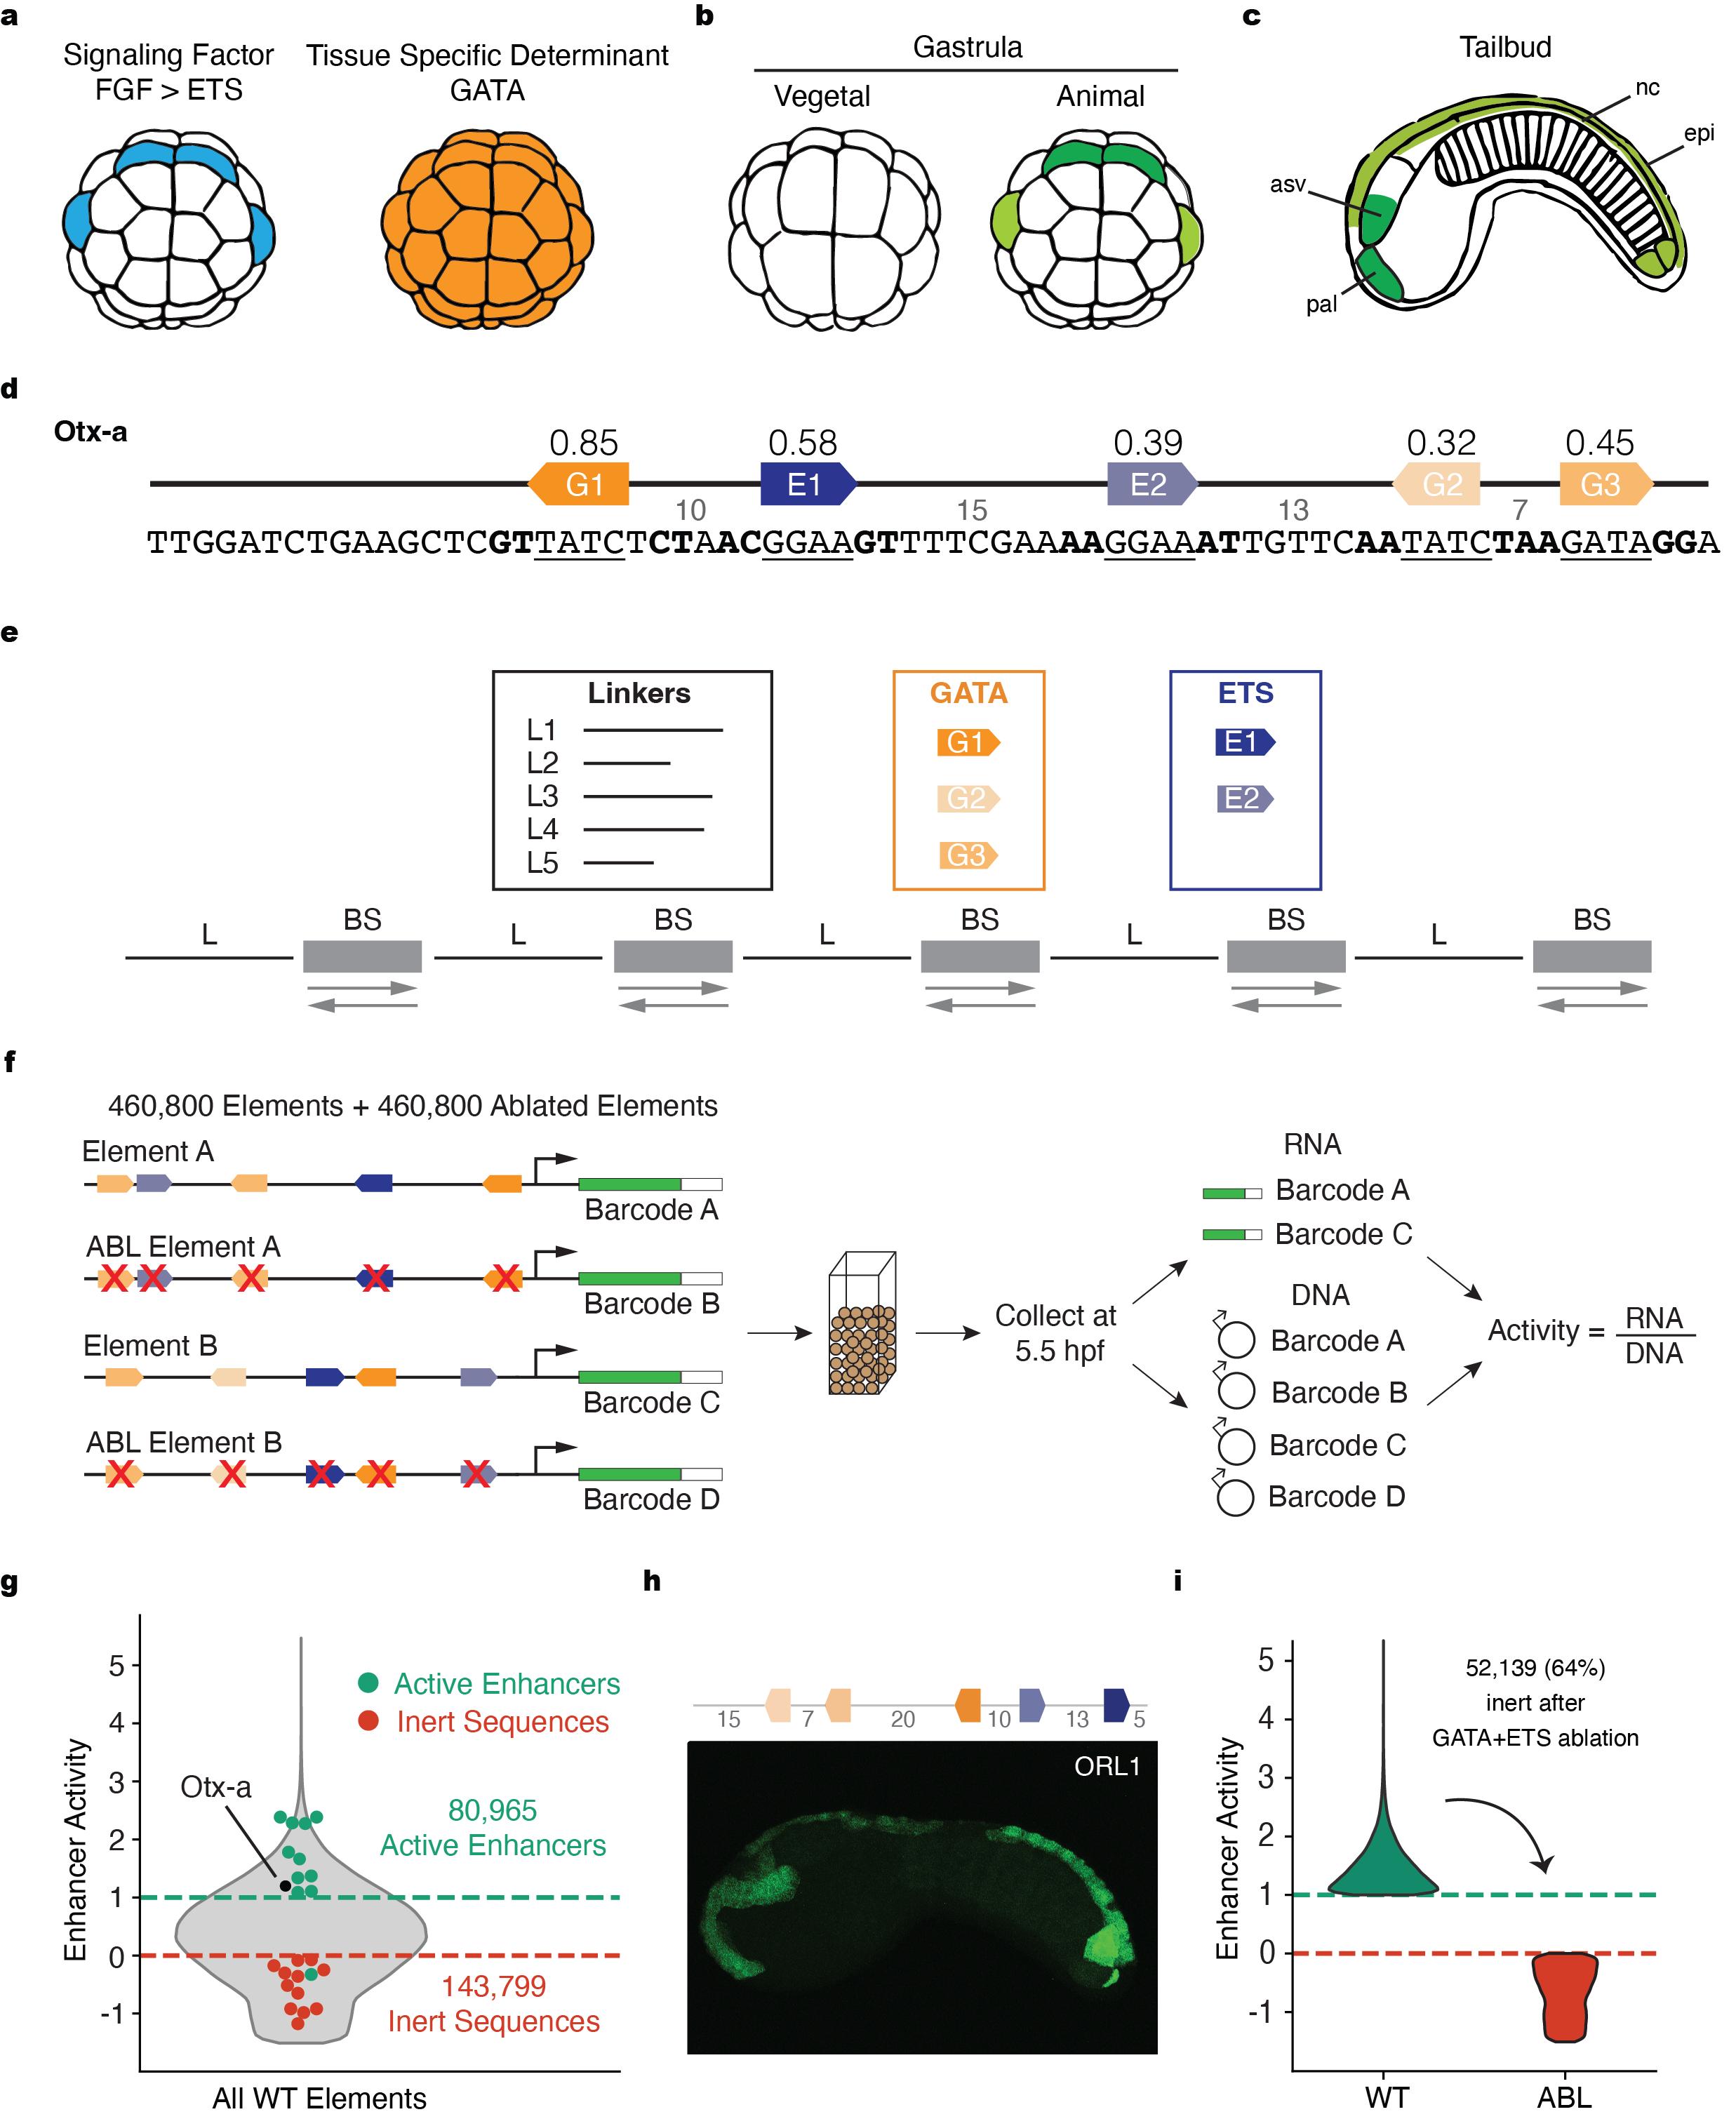
\includegraphics[height=0.8\textheight, keepaspectratio]{2_figures-and-files/Fig1.png}
    \caption[Screening every possible rearrangement of TFBSs in the \textit{Otx-a} enhancer via MPRA.]{\textbf{Screening every possible rearrangement of TFBSs in the \textit{Otx-a} enhancer via MPRA}.}
    \label{fig:2 Figure 1}
\end{figure}

\clearpage

%%%%%%%%%%%%%%%%%%%%%%%%%%%%%%%%%%%%%%%%%%%%%%%%%%%%%%%%%%%%%%%%%%%%%%%%%%%%%%%%

\subsection{TFBS syntax alone accurately predicts enhancer activity}

We next sought to build an accurate classifier of the functional enhancers in this screen. We reasoned that the 52,139 functional enhancers dependent on GATA and ETS should be predictable from the syntax of the five TFBS alone and developed a simple encoding of sequences that captures only the type, orientation and position of each TFBS core (\textbf{Figure~\ref{fig:2 Figure 2}a}, see Methods). This “syntax encoding” allows the model to flexibly learn combinations of TFBS that drive activity without having to hand-craft these features \textit{a priori}. It also eliminates the influence of any features in the linker sequences or at junctions that we do not expect to be major drivers of enhancer function in this screen.

We generated training and test data such that no two syntaxes appeared in both sets and evaluated several types of neural network classifiers that utilized the syntax encoding (\textbf{Figure~\ref{fig:2 Figure 2}b}). A convolutional neural network (CNN) with dilated convolutions and residual connections\cite{Koo2021-ly} performed best across 10-folds of cross validation (\textbf{Supplementary Figure~\ref{fig:2 supplementary_6}}), and achieved an area under the precision-recall curve (auPRC) of 0.59 on held-out test data (\textbf{Figure~\ref{fig:2 Figure 2}c}). We call this model Sirius in homage to its canine-named predecessors\cite{Kelley2016-oh,Gosai2023-cw}.

We found that Sirius’s performance was not dependent on using only active enhancers driven by GATA and ETS and that including the full set of 80,965 active enhancers as positives led to almost identical predictions and performance (\textbf{Supplementary Figure~\ref{fig:2 supplementary_7}}). Including affinity (\textbf{Figure~\ref{fig:2 Figure 2}c}, Sirius + Affinity) led to only a marginal increase in performance, indicating that placement of sites with differing affinities plays a relatively small role in this screen compared to syntax. We also evaluated Sirius’s ability to predict the continuous MPRA activity level using the raw scores produced by the model (see Methods). Despite being trained on binary labels, we found a modest correlation with activity level (\textbf{Supplementary Figure~\ref{fig:2 supplementary_7}}). Surprisingly, training models to directly predict continuous activity levels from all detected sequences in a regression setting yielded comparable performance (\textbf{Supplementary Figure~\ref{fig:2 supplementary_7}}). 

We designed the syntax encoding to ensure the spurious features are ignored by the model, but it is possible that the linear DNA sequence contains bona fide learnable features (e.g., flanks or de novo sites). We therefore benchmarked sequence-based models on the same task (\textbf{Figure~\ref{fig:2 Figure 2}c}, \textbf{Supplementary Figure~\ref{fig:2 supplementary_8}a}, \textbf{Supplementary Figure~\ref{fig:2 supplementary_8}b})\cite{Ghandi2014-ql}. A model trained on sequence of the same architecture (SiriusSeq) outperformed Sirius, but the relatively small improvement highlights that most of the information needed to predict activity is present in the TFBS cores. The performance of SiriusSeq was only slightly higher than Sirius + Affinity, suggesting that the additional predictive information in the sequence comes from the flanks. To directly test which sequence features SiriusSeq prioritized, we evaluated test set performance on sequences in which we randomized different features (\textbf{Figure~\ref{fig:2 Figure 2}d}, \textbf{Supplementary Figure~\ref{fig:2 supplementary_8}c}). We observed that the randomization of linker sequences led to a drop in predictive accuracy of similar magnitude to randomization of TFBS cores. Motif enrichment analysis from model-derived features (see Methods) pinpointed several motifs resembling sites with flanking nucleotides, and did not detect any known de novo motifs (\textbf{Supplementary Figure~\ref{fig:2 supplementary_8}d}, \textbf{Supplementary Table 2}). Taken together, these results suggest that syntax alone is enough to build an accurate and robust predictor of enhancer function from this screen, and that the additional information present in flanks and linkers has a relatively small contribution to enhancer function.

\clearpage

\thispagestyle{plain}
\noindent
\textbf{Figure~\ref{fig:2 Figure 2}. A convolutional neural network trained on TFBS syntax accurately discriminates inert sequences from active enhancers}. a) Syntax encoding schematic. Each library member is encoded by the position of GATA and ETS sites in both forward and reverse orientations, capturing order, orientation and spacing of the sites (see Methods). b) Machine learning model training schematic. Library members are partitioned into training, validation and test sets (see Methods). Training sequences are syntax encoded and used to train neural networks. Model predictions are continuous values that are transformed to probabilities via the sigmoid function and compared to MPRA labels to assess classification performance. c) Precision-recall curves for syntax encoding (Sirius), syntax + affinity encoding (Sirius + Affinity) and sequence (SiriusSeq) on held-out test data. Area under the curve (auPRCs) are indicated in parentheses. The dashed grey line indicates the performance of a random classifier. d) SiriusSeq held-out test set auPRCs on sequences with the indicated randomized features.

\clearpage

\begin{figure}[!htbp]
    \centering
    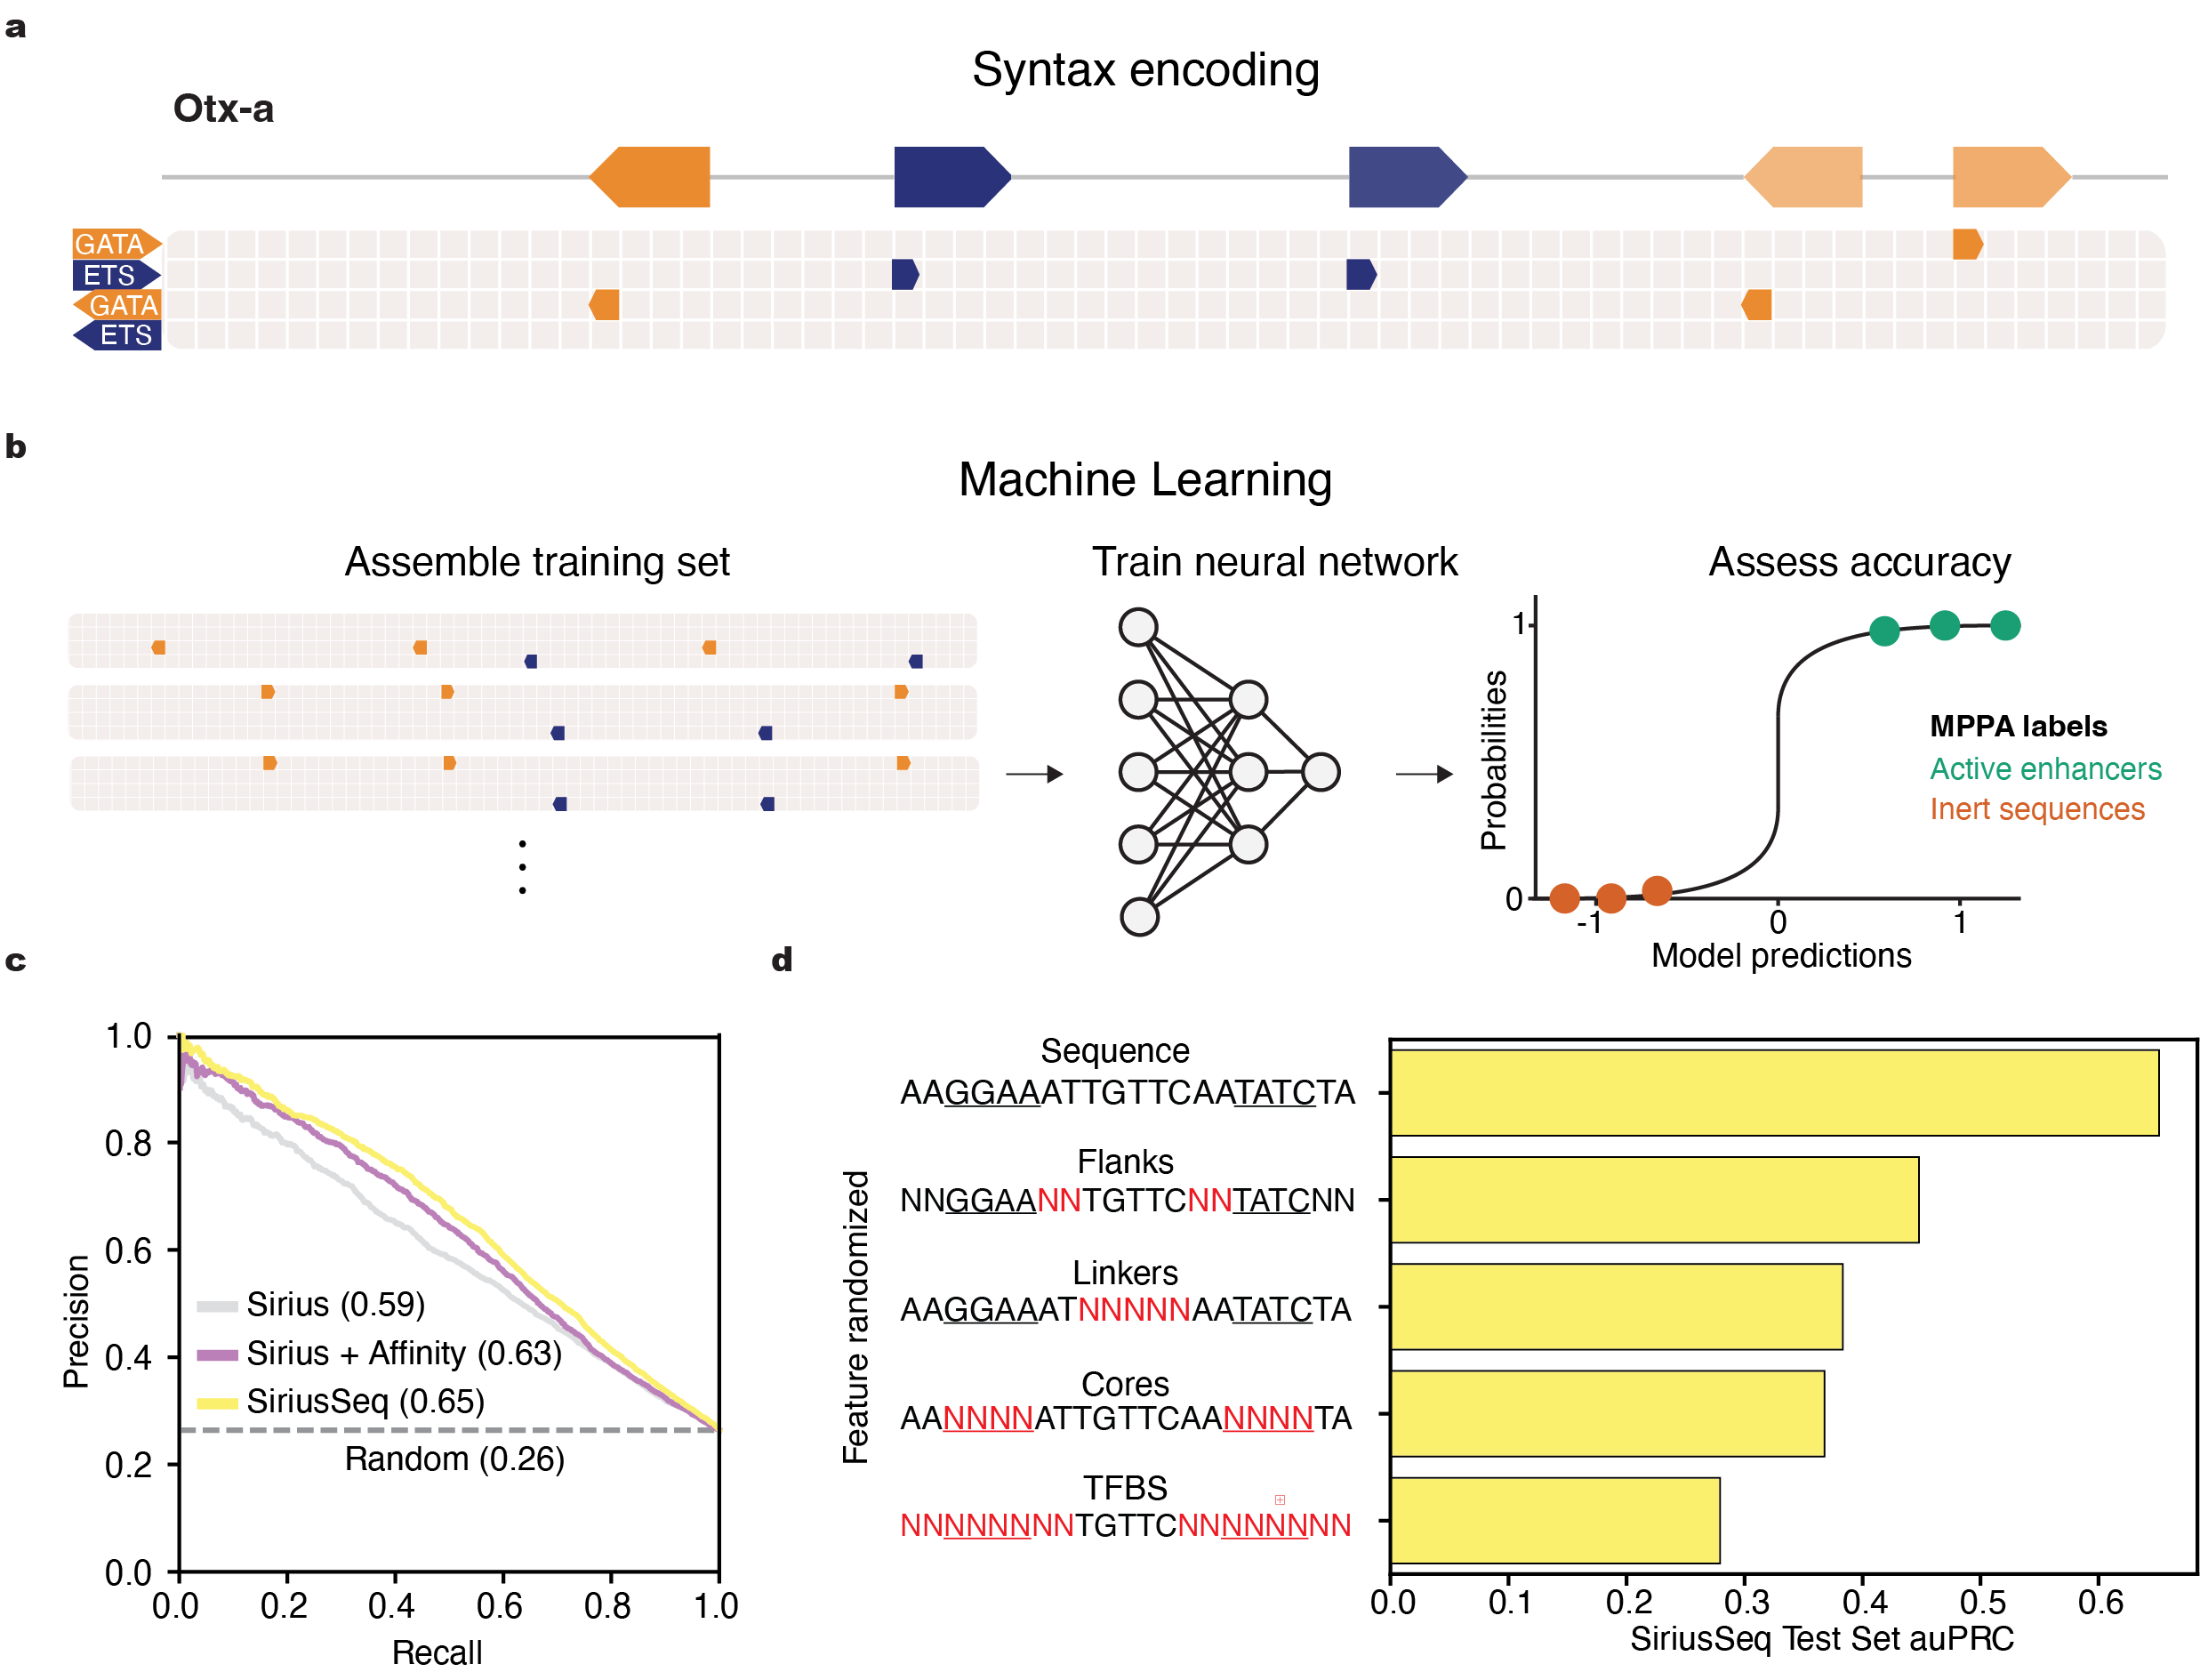
\includegraphics[height=0.7\textheight, keepaspectratio]{2_figures-and-files/Fig2.png}
    \caption[A convolutional neural network trained on TFBS syntax accurately discriminates inert sequences from active enhancers.]{\textbf{A convolutional neural network trained on TFBS syntax accurately discriminates inert sequences from active enhancers}.}
    \label{fig:2 Figure 2}
\end{figure}

\clearpage

%%%%%%%%%%%%%%%%%%%%%%%%%%%%%%%%%%%%%%%%%%%%%%%%%%%%%%%%%%%%%%%%%%%%%%%%%%%%%%%%

\subsection{Sirius learns a primarily additive model of TFBS syntax features}

Identification of TFBS syntax rules that govern enhancer function remains a central challenge in regulatory genomics\cite{Jindal2021-zk}. Although neural networks are often viewed as black boxes, methods for interpreting trained models can reveal the sequence features they prioritize and help us better understand how they arrive at their predictions\cite{Novakovsky2022-ft}. To investigate the most significant features in our screen, we systematically analyzed patterns of two and three binding sites, referred to here as organizational features (see Methods), and measured their impact on model predictions by marginalizing them across all the syntaxes they occurred in (\textbf{Figure~\ref{fig:2 Figure 3}a}). This yielded 15 significantly inactivating and 23 significantly activating 2-site features, as well as 654 inactivating and 1005 activating 3-site features (\textbf{Figure~\ref{fig:2 Figure 3}b}), which we refer to collectively as syntax features. We found that both activating 2-site and 3-site features were enriched for configurations containing two ETS sites (\textbf{Supplementary Figure~\ref{fig:2 supplementary_9}a}), highlighting the importance of the proper configuration of ETS sites in functional syntaxes. Activating syntax features preferentially occurred toward the downstream half of the 66bp sequence, while inactivating features showed a slight positional skew upstream (\textbf{Supplementary Figure~\ref{fig:2 supplementary_9}b}). Additionally, a subset of 2-site features exhibited periodic positional preferences, potentially reflecting helical phasing constraints or other spacing-related syntax rules (\textbf{Supplementary Figure~\ref{fig:2 supplementary_9}c}).

To validate predicted syntax features, we first experimentally tested two in which we observed strong predicted activating effects. We synthesized sequences containing only a single instance of each syntax feature and assayed their activity \textit{in vivo} using fluorescence microscopy. Both sequences drove \textit{Otx-a} WT like expression, consistent with their predicted activating function (\textbf{Figure~\ref{fig:2 Figure 3}c}). We also observed several instances where subtle changes in 3-site syntax features create opposite directions of effect (\textbf{Supplementary Figure~\ref{fig:2 supplementary_9}d}). For instance, the organizational feature g.14.e.8.g is predicted to be an inactivating syntax feature (\textbf{Figure~\ref{fig:2 Figure 3}d}, left), but when the central ETS site is flipped to the forward strand, it is predicted to be activating (\textbf{Figure~\ref{fig:2 Figure 3}d}, right). Consistent with model predictions, a syntax containing the inactivating variant showed no activity, while the same syntax with only the ETS site flipped showed \textit{Otx-a} WT like expression (\textbf{Figure~\ref{fig:2 Figure 3}d}).

To better understand how the model combines the individual effects of syntax features to make its final prediction, we designed an additive model that sums the effect sizes of all organizational features present in a given sequence (\textbf{Figure~\ref{fig:2 Figure 3}e}, AdditiveFeatures). This additive model explained 56\% of the variance in the predictions made by Sirius (\textbf{Supplementary Figure~\ref{fig:2 supplementary_9}e}) and captures approximately 81\% of the gain in its predictive performance compared to a random classifier (\textbf{Figure~\ref{fig:2 Figure 3}f}). This suggests that a large portion of the model’s predictive capacity is driven by the independent contributions of individual syntax features it has learned to prioritize. While non-linear interactions between these features likely exist, they play a relatively minor role compared to linear ones.

\clearpage
\thispagestyle{plain}
\noindent
\textbf{Figure~\ref{fig:2 Figure 3}.} \textbf{Sirius combines syntax-features in a primarily additive model}. a) Schematic for organizational feature marginalization analysis. Each of 9,022 2-site and 3-site organizational features (see Methods) is tested by splitting up all 460,800 sequences in the library into those that do not contain the feature (No Feature) and those that do (Contains Feature). A Mann-Whitney U-test on the distribution of model predictions for the two groups is used to assign statistical significance (corrected with Benjamini-Hochberg method) and the relative log-odds of mean predictions between groups is used to define an effect size. b) Volcano plots for 2-site (left) and 3-site (right) syntax features where the x-axis shows log2 of the mean relative odds predicted by the model and the y-axis shows -log10(corrected p-value) from the Mann-Whitney U-Test in a). Organizational features are colored based on whether their adjusted p-value is < 0.01 and log2 relative odds is greater than 1 (activating, doubling of odds) or less than -1 (inactivating, halving of odds). c) Two 3-site syntax features that are predicted to be strongly activating act as synthetic active enhancers. d) A single strand flip of an ETS site in a 3-site syntax feature turns it from inactivating (left) to activating (right). e) Schematic for generating a AdditiveFeature score for the \textit{Otx-a} WT sequence (see Methods). The mean relative odds for each organizational feature contained in the sequence are summed. f) Test set precision-recall curves of AdditiveFeature model compared to full syntax model (Sirius) and random classifier. Numbers in parentheses indicate area under the precision-recall curve (auPRC).

\clearpage

\begin{figure}[!htbp]
    \centering
    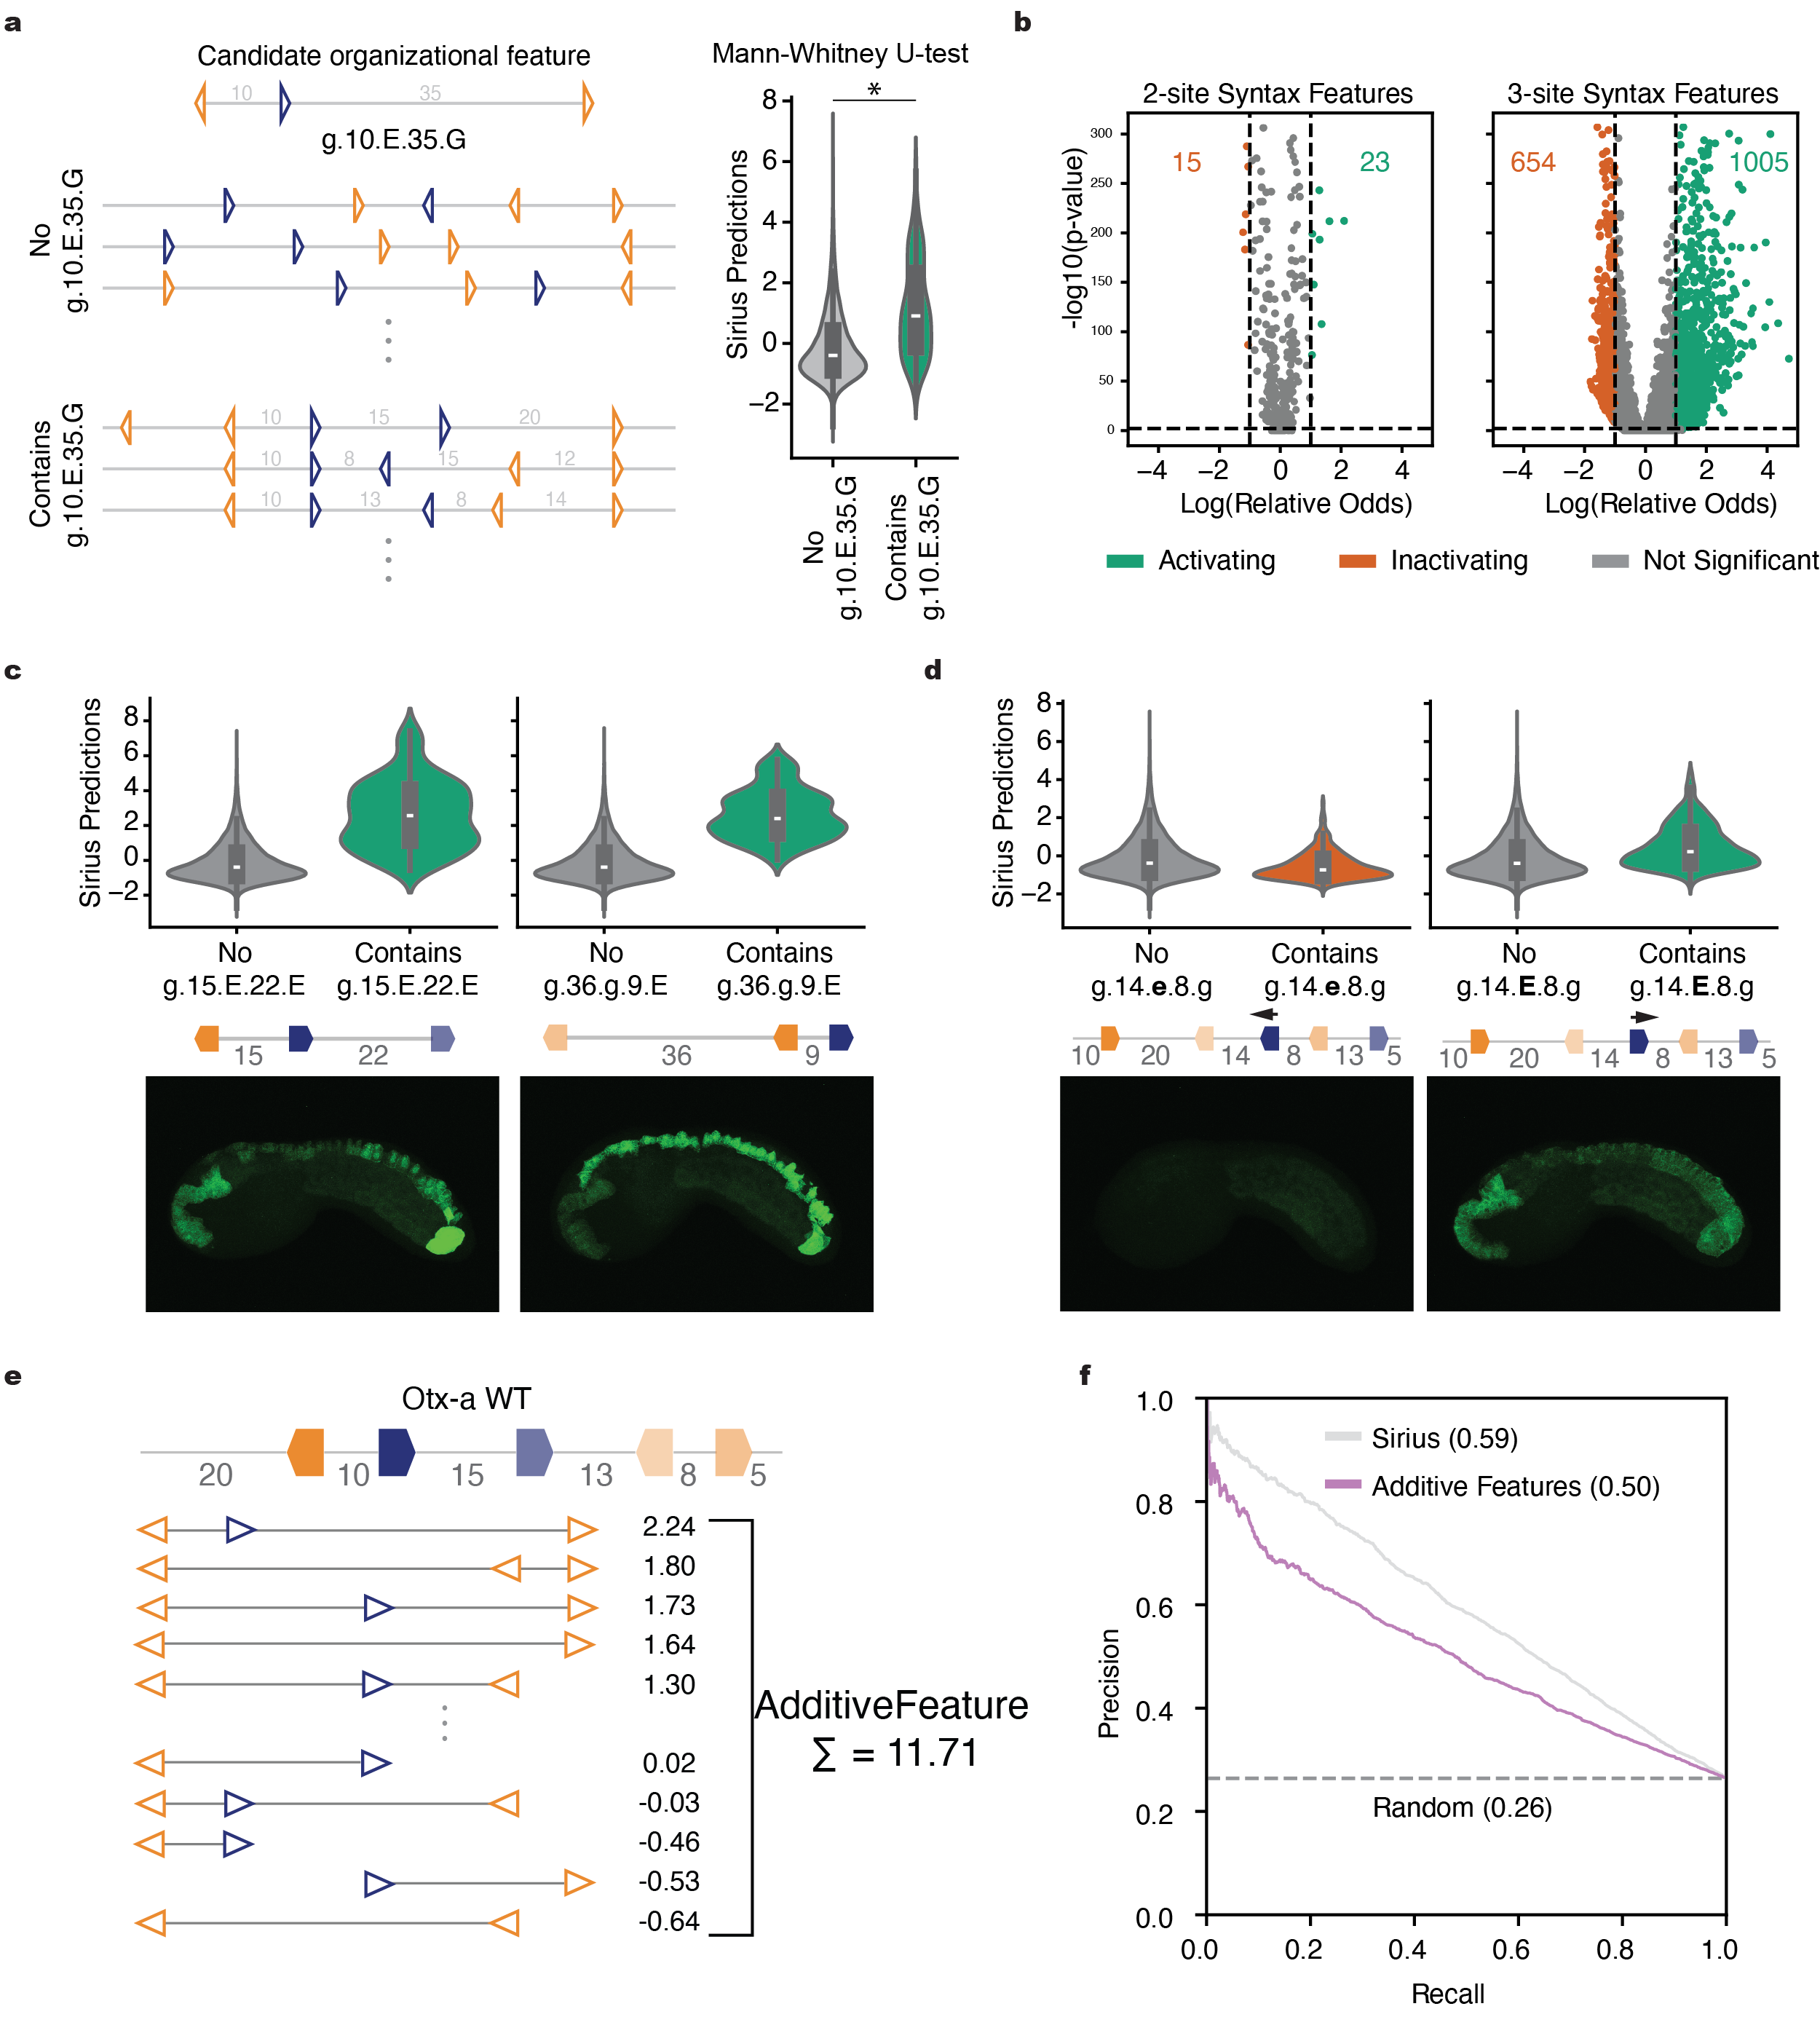
\includegraphics[height=0.75\textheight, keepaspectratio]{2_figures-and-files/Fig3.png}
    \caption[Sirius combines syntax-features in a primarily additive model.]{\textbf{Sirius combines syntax-features in a primarily additive model}.}
    \label{fig:2 Figure 3}
\end{figure}

\clearpage

%%%%%%%%%%%%%%%%%%%%%%%%%%%%%%%%%%%%%%%%%%%%%%%%%%%%%%%%%%%%%%%%%%%%%%%%%%%%%%%%

\subsection{Sirius enables tissue-specific enhancer design}

Of the sequences we validated using fluorescence microscopy, several showed activity in tissues other than the neural lineages expected for the WT \textit{Otx-a} enhancer (\textbf{Supplementary Figure~\ref{fig:2 supplementary_10}a}, \textbf{Supplementary Figure~\ref{fig:2 supplementary_10}b}). Sirius predictions for these “ectopic enhancers” were higher than those for neural-specific active enhancers (neural enhancers) (\textbf{Supplementary Figure~\ref{fig:2 supplementary_10}a}). To assess this more systematically, we categorized all the library sequences into three groups: 1) inert sequences, 2) neural enhancers and 3) ectopic enhancers, using a combination of MPRA activity and two other metrics previously shown to be predictive of tissue specificity. These three groups were well separated by Sirius predictions across models trained on different folds (\textbf{Supplementary Figure~\ref{fig:2 supplementary_10}c}, \textbf{Supplementary Figure~\ref{fig:2 supplementary_10}d}).

Inspired by previous work on synthetic enhancer design using neural networks\cite{Taskiran2023-xz,Gosai2023-cw}, we developed a strategy to design synthetic enhancers using Sirius (\textbf{Figure~\ref{fig:2 Figure 4}a}). The design process begins with a starting sequence for which we then select one of four possible “syntax edits” at random. A syntax edit is a perturbation made to the sequence that operates at the level of TFBS rather than the linear DNA sequence. Each type of syntax edit generates a set of candidate syntaxes, which we then score using a scoring function based on Sirius predictions, often the distance from a prespecified target value. Selecting the highest-scoring sequence from the pool of candidates generates a new starting point for another iteration of design. We continue this process for a set number of iterations or until a convergence threshold is reached. In this way, the model can be used to generate synthetic enhancers.

To test whether Sirius could design sequences with tissue specificity, we chose an objective function which minimizes the difference between Sirius predictions and the median of the neural enhancer group (\textbf{Supplementary Figure~\ref{fig:2 supplementary_10}c}). We call the sequences generated by this process STARS (Syntax-derived, Tissue-specific, Active Regulatory Sequences). We selected 16 starting syntaxes from our microscope-validated set to design neural enhancers from (\textbf{Supplementary Figure~\ref{fig:2 supplementary_10}b}), 14 are inert syntaxes that represent candidates for activating STARS and 2 are ectopic syntaxes that represent candidates for tuned STARS. For each starting syntax, we performed 25 rounds of design across multiple random seeds and selected STARS (see Methods). We generated single activated STARS from each of the 14 starting inert sequences (\textbf{Figure~\ref{fig:2 Figure 4}b}, \textbf{Supplementary Figure~\ref{fig:2 supplementary_11}a}) and five tuned STARS for each of the two starting ectopic sequences (tuned STARS) (\textbf{Figure~\ref{fig:2 Figure 4}c}, \textbf{Supplementary Figure~\ref{fig:2 supplementary_11}b}).

We then generated a library of sequences based on these 24 total STARS to experimentally validate via MPRA. For each of the STARS, we generated a total of 8 sequences by varying the composition of the flanks and linkers between the sites (\textbf{Supplementary Figure~\ref{fig:2 supplementary_12}}, see Methods). The final STARS library contained 421 unique sequences: 192 synthetic designs, a set of 192 ablated controls for each design, and 37 sequences from the OSL library controls. We split the sequences into two libraries to improve the signal to noise ratio, keeping the same set of 37 controls in each library. 

We electroporated both libraries into \textit{Ciona} embryos and quantified enhancer activity using the ratio of detected RNA barcodes to plasmid copy number for each sequence. Replicate concordance was high across the controls shared between libraries (\textbf{Supplementary Figure~\ref{fig:2 supplementary_13}a}). We again used a set of microscope-validated controls to determine activity thresholds classifying sequences as inert sequences, neural enhancers or ectopic enhancers (\textbf{Supplementary Figure~\ref{fig:2 supplementary_13}b}, \textbf{Supplementary Figure~\ref{fig:2 supplementary_13}c}, see Methods). Nearly all ablated sequences were inactive (190/192), indicating that the syntax of GATA and ETS sites drives activity for the sequences in this library (\textbf{Supplementary Figure~\ref{fig:2 supplementary_13}b}, \textbf{Supplementary Figure~\ref{fig:2 supplementary_13}c}). Among the activated STARS, 92\% (103/112) showed increased activity relative to their starting syntax, with 67\% (75/112) classified as active enhancers and 71\% (53/75) of those further classified as neural enhancers (\textbf{Figure~\ref{fig:2 Figure 4}d}). For tuned STARS, 95\% (76/80) decreased in activity, with 90\% (72/80) classified as either inert sequences or neural enhancers and 50\% (36/72) of those as neural enhancers (\textbf{Figure~\ref{fig:2 Figure 4}e}). Finally, SiriusSeq predictions across the STARS libraries showed a moderate but statistically significant correlation with MPRA activity and enhancer class labels (\textbf{Supplementary Figure~\ref{fig:2 supplementary_14}}). In sum, these results demonstrate that a syntax-based design approach can be used to generate synthetic enhancers with tunable and tissue-specific activity.

\clearpage

\thispagestyle{plain}
\noindent
\textbf{Figure~\ref{fig:2 Figure 4}. Syntax-driven design of tissue-specific synthetic enhancers}. a) Schematic of design process. We define four types of syntax edit that each generate a set of candidate syntaxes to score with the model. In each round of design, a syntax edit type is selected at random and candidate syntaxes are generated. Activity is then predicted with Sirius and transformed to a score using a chosen objective function. The highest scoring syntax is then selected for the next round of editing. Examples of activated (b) and tuned (c) STARS. Left, binding site syntaxes of sequences at each round. Right, model prediction for each round. Background colors are determined by the interquartile ranges of the Inert Sequence, Neural Enhancer and Ectopic Enhancer distributions shown in \textbf{Supplementary Figure~\ref{fig:2 supplementary_10}}c. STARS MPRA analysis for activated e) and tuned f) STARS. Y-axis shows change in measured activity of the designed sequence with respect to the measured activity of its starting sequence. Each syntax was used to generate eight different DNA sequences with differing flanks and linkers. Each point (sequence) is colored by the classification label assigned using thresholds from internal controls validated with fluorescence microscopy (\textbf{Supplementary Figure~\ref{fig:2 supplementary_13}}b,c). Barplot on top indicates the number of GATA and ETS sites in the respective designed syntax.

\clearpage

\begin{figure}[!htbp]
    \centering
    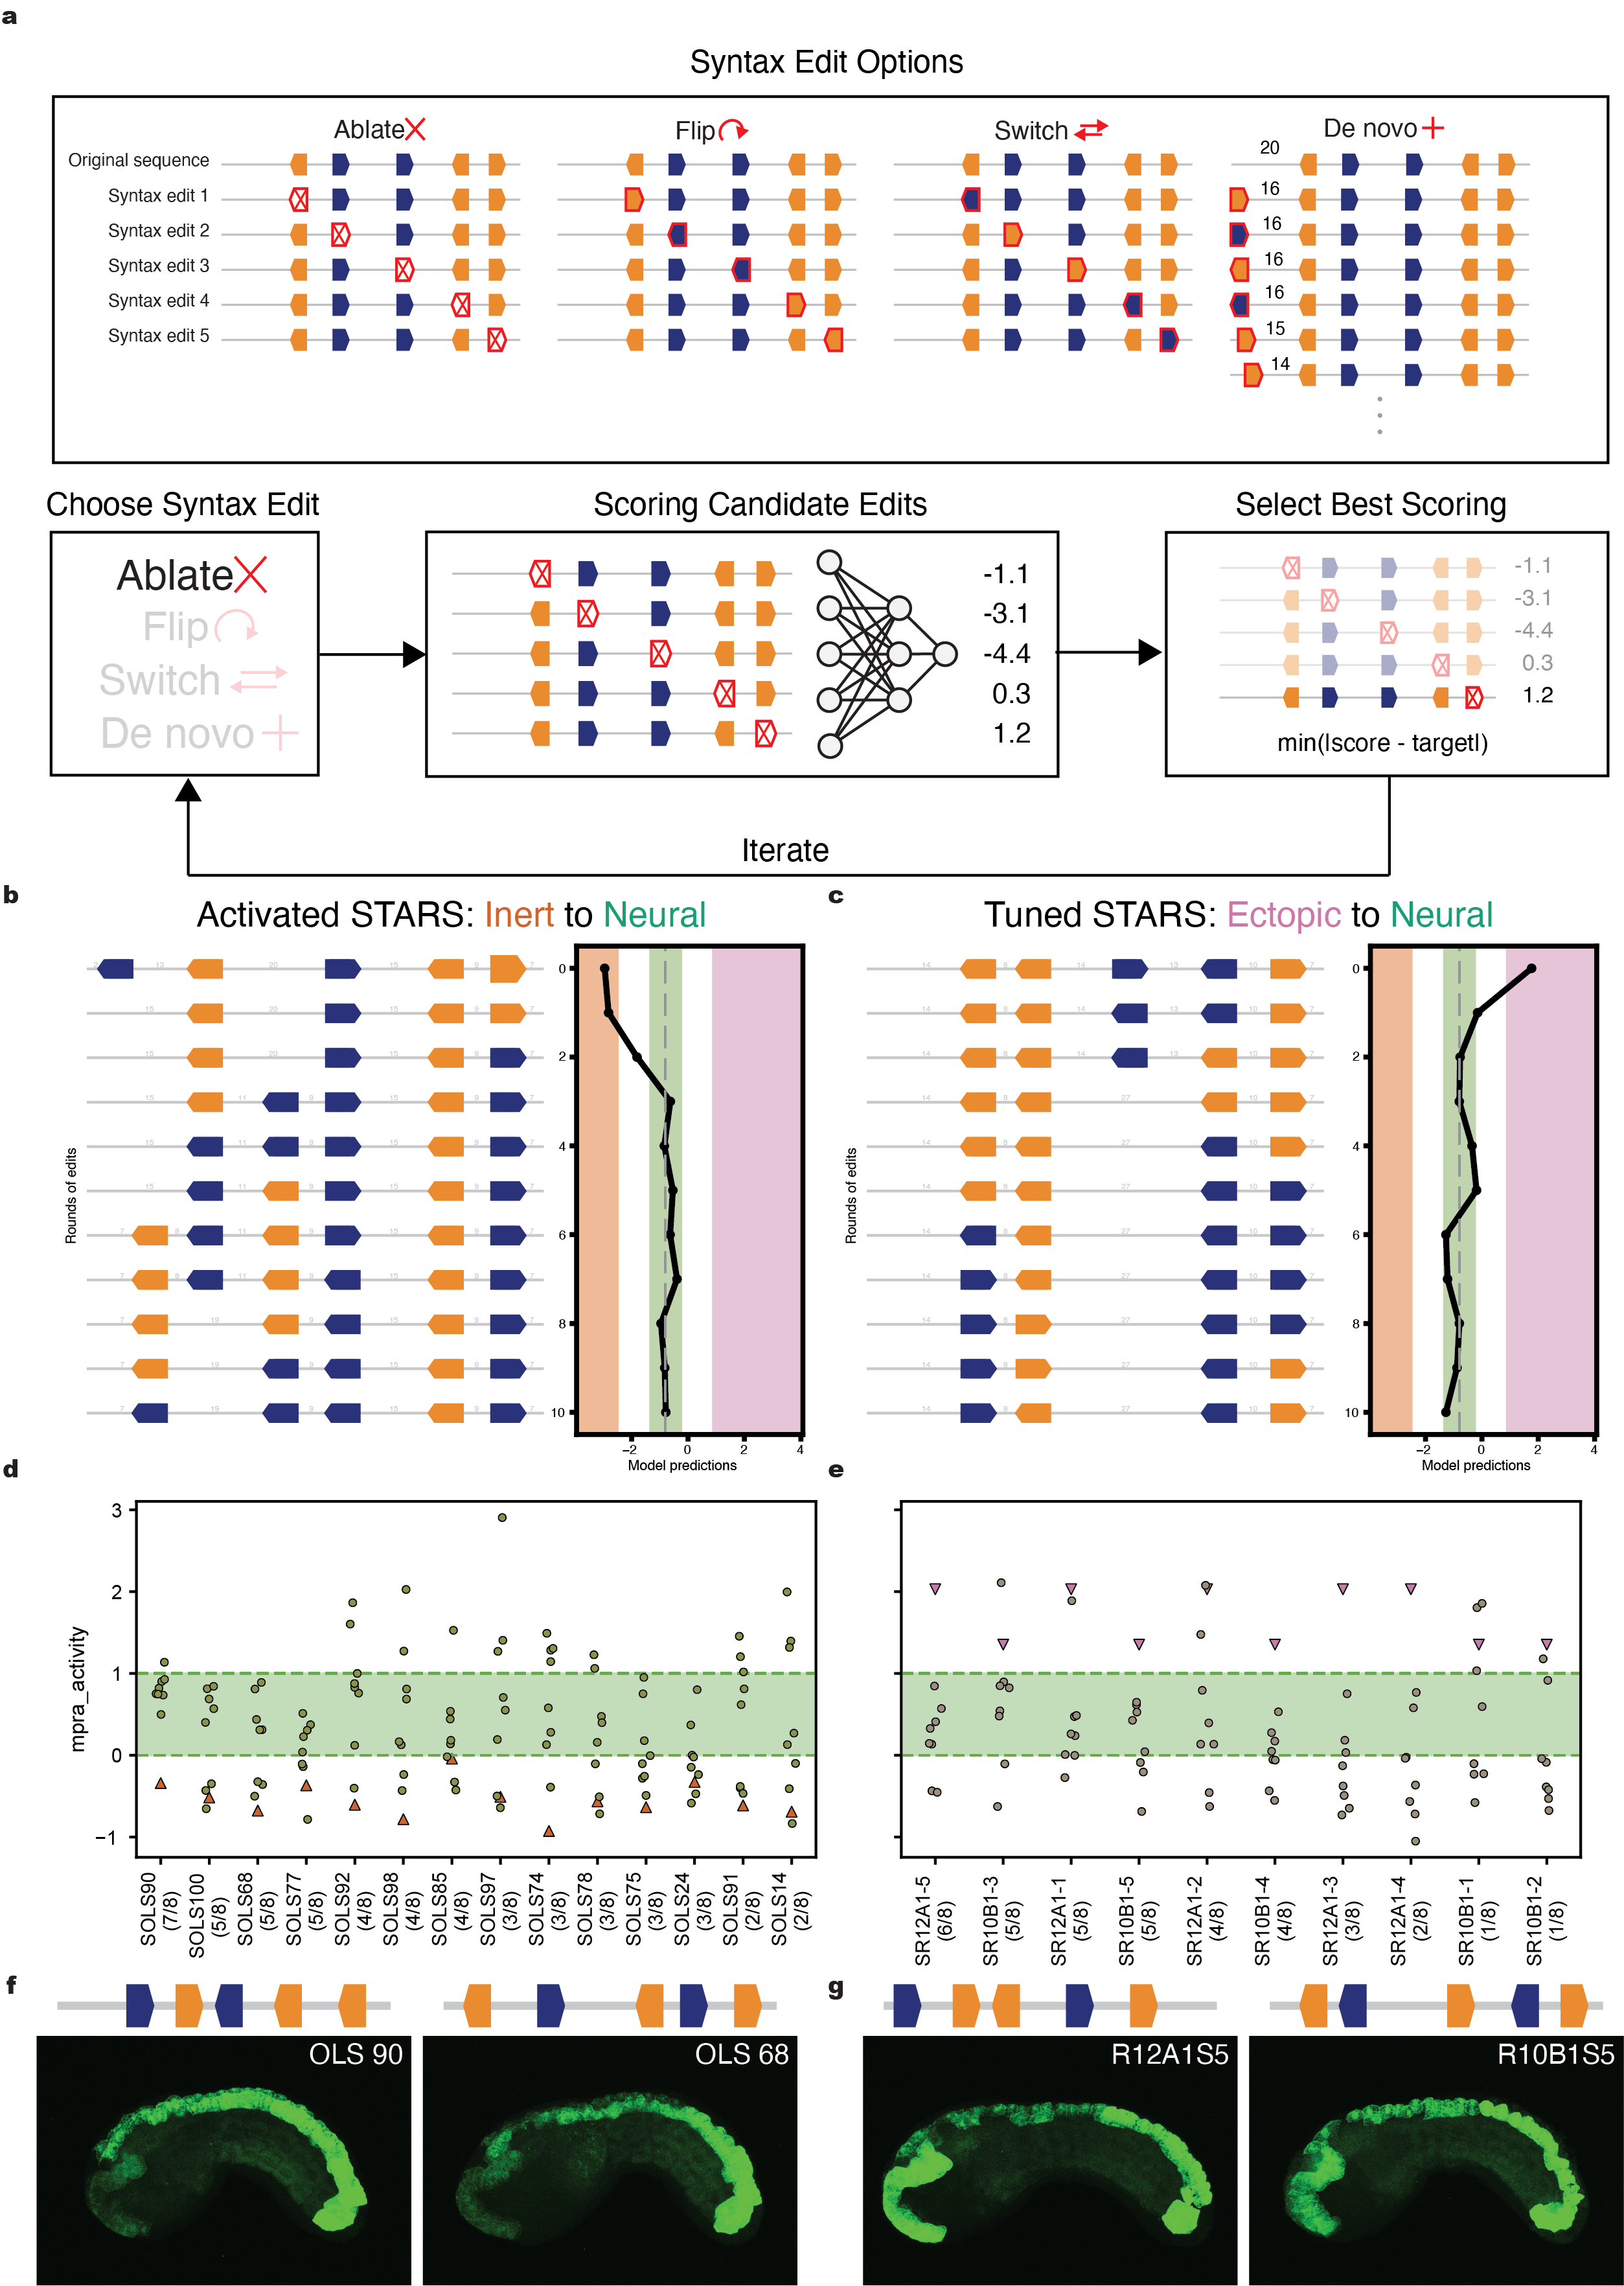
\includegraphics[height=0.75\textheight, keepaspectratio]{2_figures-and-files/Fig4.png}
    \caption[Syntax-driven design of tissue-specific enhancers.]{\textbf{Syntax-driven design of tissue-specific enhancers}.}
    \label{fig:2 Figure 4}
\end{figure}

\clearpage

%%%%%%%%%%%%%%%%%%%%%%%%%%%%%%%%%%%%%%%%%%%%%%%%%%%%%%%%%%%%%%%%%%%%%%%%%%%%%%%%

\subsection{Features beyond GATA/ETS syntax improve prediction of genomic enhancer function}

Clusters of ETS and GATA sites are widespread in the genome, but their regulatory potential is largely uncharacterized. We therefore created a sequence library from 66bp genomic elements that contain at least one ETS (>0.1 relative affinity), one GATA (>0.2 relative affinity) site, and a total of three or four sites (\textbf{Figure~\ref{fig:2 Figure 5}a}). This totaled 3,318 genomic elements, which we electroporated into \textit{Ciona} embryos and tested their activity via MPRA (\textbf{Figure~\ref{fig:2 Figure 5}b}, see Methods). We included six control sequences (including \textit{Otx-a} WT) with known expression patterns to establish thresholds for classifying active enhancers from inert sequences. We find that 1,148 of the genomic elements drive expression with levels similar to or greater than \textit{Otx-a} WT, and that 1,840 are inert (\textbf{Figure~\ref{fig:2 Figure 5}b}). The remaining 330 elements show very weak enhancer activity.

We first asked whether individual features could distinguish active enhancers from inert genomic sequences. Neither the number of sites (\textbf{Supplementary Figure~\ref{fig:2 supplementary_15}a}) nor the affinity of ETS sites (\textbf{Supplementary Figure~\ref{fig:2 supplementary_15}b}) differed significantly between active enhancers and inert sequences. In contrast, active enhancers tended to have modestly higher GATA site affinity than inert sequences (\textbf{Supplementary Figure~\ref{fig:2 supplementary_15}c}). Models trained on the OSL library showed only modest performance gains over a random classifier (auPRC = 0.38), of which Sirius was the highest (auPRC = 0.44) (\textbf{Figure~\ref{fig:2 Figure 5}d}). When stratified by aggregated affinity for each type of site, we observed an increase in the percentage of active enhancers for elements with strong syntax (top 20th percentile of Sirius predictions) relative to elements without syntax (bottom 20th percentile of Sirius predictions) (\textbf{Figure~\ref{fig:2 Figure 5}d}). We noted the strongest increase in three particular bins: 1) elements with high ETS affinity and low GATA affinity, 2) elements with high ETS affinity and high GATA affinity, and 3) elements with low ETS affinity bins and moderate GATA affinity.

The relatively modest predictive capability of these OSL trained models suggests that predictive features outside of those contained in the OSL library are present in the tested genomic clusters. Indeed, models trained directly on genomic sequences (Genomic Sequence) performed better than Sirius (\textbf{Supplementary Figure~\ref{fig:2 supplementary_15}d}), albeit with large variability across three folds, likely due to the sample size. We found that fine-tuning models trained first on the OSL library led to more reproducible performance, at the cost of some predictive power (\textbf{Supplementary Figure~\ref{fig:2 supplementary_15}d}). Fine-tuned sequence models had the highest mean test set performance across three folds (\textbf{Supplementary Figure~\ref{fig:2 supplementary_15}d}), with fine-tuned syntax and syntax + affinity models showing lower overall performance, but similar performance to each other.

To test whether our approach to modeling enhancer function based on TFBS syntax is generalizable beyond the \textit{Ciona} system, we analyzed data from a study of four core pluripotency transcription factors: Oct4, Sox2, Klf4, and Esrrb in mouse embryonic stem cells (mESCs)\cite{King2020-hk}. We first trained a Sirius-style model on a syntax encoding of the synthetic MPRA conducted in that study, achieving accurate quantitative predictions (R\textsuperscript{2} = 0.92) and a 6\% increase in performance over the published random forest model (R\textsuperscript{2} = 0.87) trained on hand-crafted features (\textbf{Supplementary Figure~\ref{fig:2 supplementary_16}a}). We also trained a Syntax + Affinity model on the genomic MPRA performed in the same study and achieved performance (auPRC = 0.82) exceeding the published gkm-SVM trained DNA sequence (auPRC = 0.77) (\textbf{Supplementary Figure~\ref{fig:2 supplementary_16}b}).

\clearpage

\thispagestyle{plain}
\noindent
\textbf{Figure~\ref{fig:2 Figure 5} OSL models predict activity of genomic clusters of ETS and GATA sites}. a) Schematic showing search for clusters of ETS and GATA binding sites. Each element contains at least one GATA site (relative affinity > 0.2) and one ETS site (relative affinity > 0.1). b) Enhancer activity of the 3,318 genomic elements tested in Ciona embryos. 1,148 elements are active enhancers while 1,840 elements are inert sequences. Activity of six internal controls are shown as the colored points: \textit{Otx-a} (black), three positive controls (green), and two negative controls (red). c) Precision-recall curves for OSL trained models on genomic clusters: Syntax encoding (Sirius), syntax + affinity encoding (Sirius + Affinity) and sequence (SiriusSeq). Areas under the curve (auPRCs) are indicated in parentheses. The dashed grey line indicates the performance of a random classifier. d) Percent of active enhancers within each group separated based on affinity and syntax. Each element is placed in a bin based on the summed affinity of ETS (heatmap Y-axis), summed affinity of GATA (heatmap X-axis) and the syntax group. Top heatmap contains elements with in the bottom 20th percentile of Sirius scores. Lower heatmap contains the elements in the top 20th percentile of Sirius scores.

\clearpage

\begin{figure}[p]
    \centering
    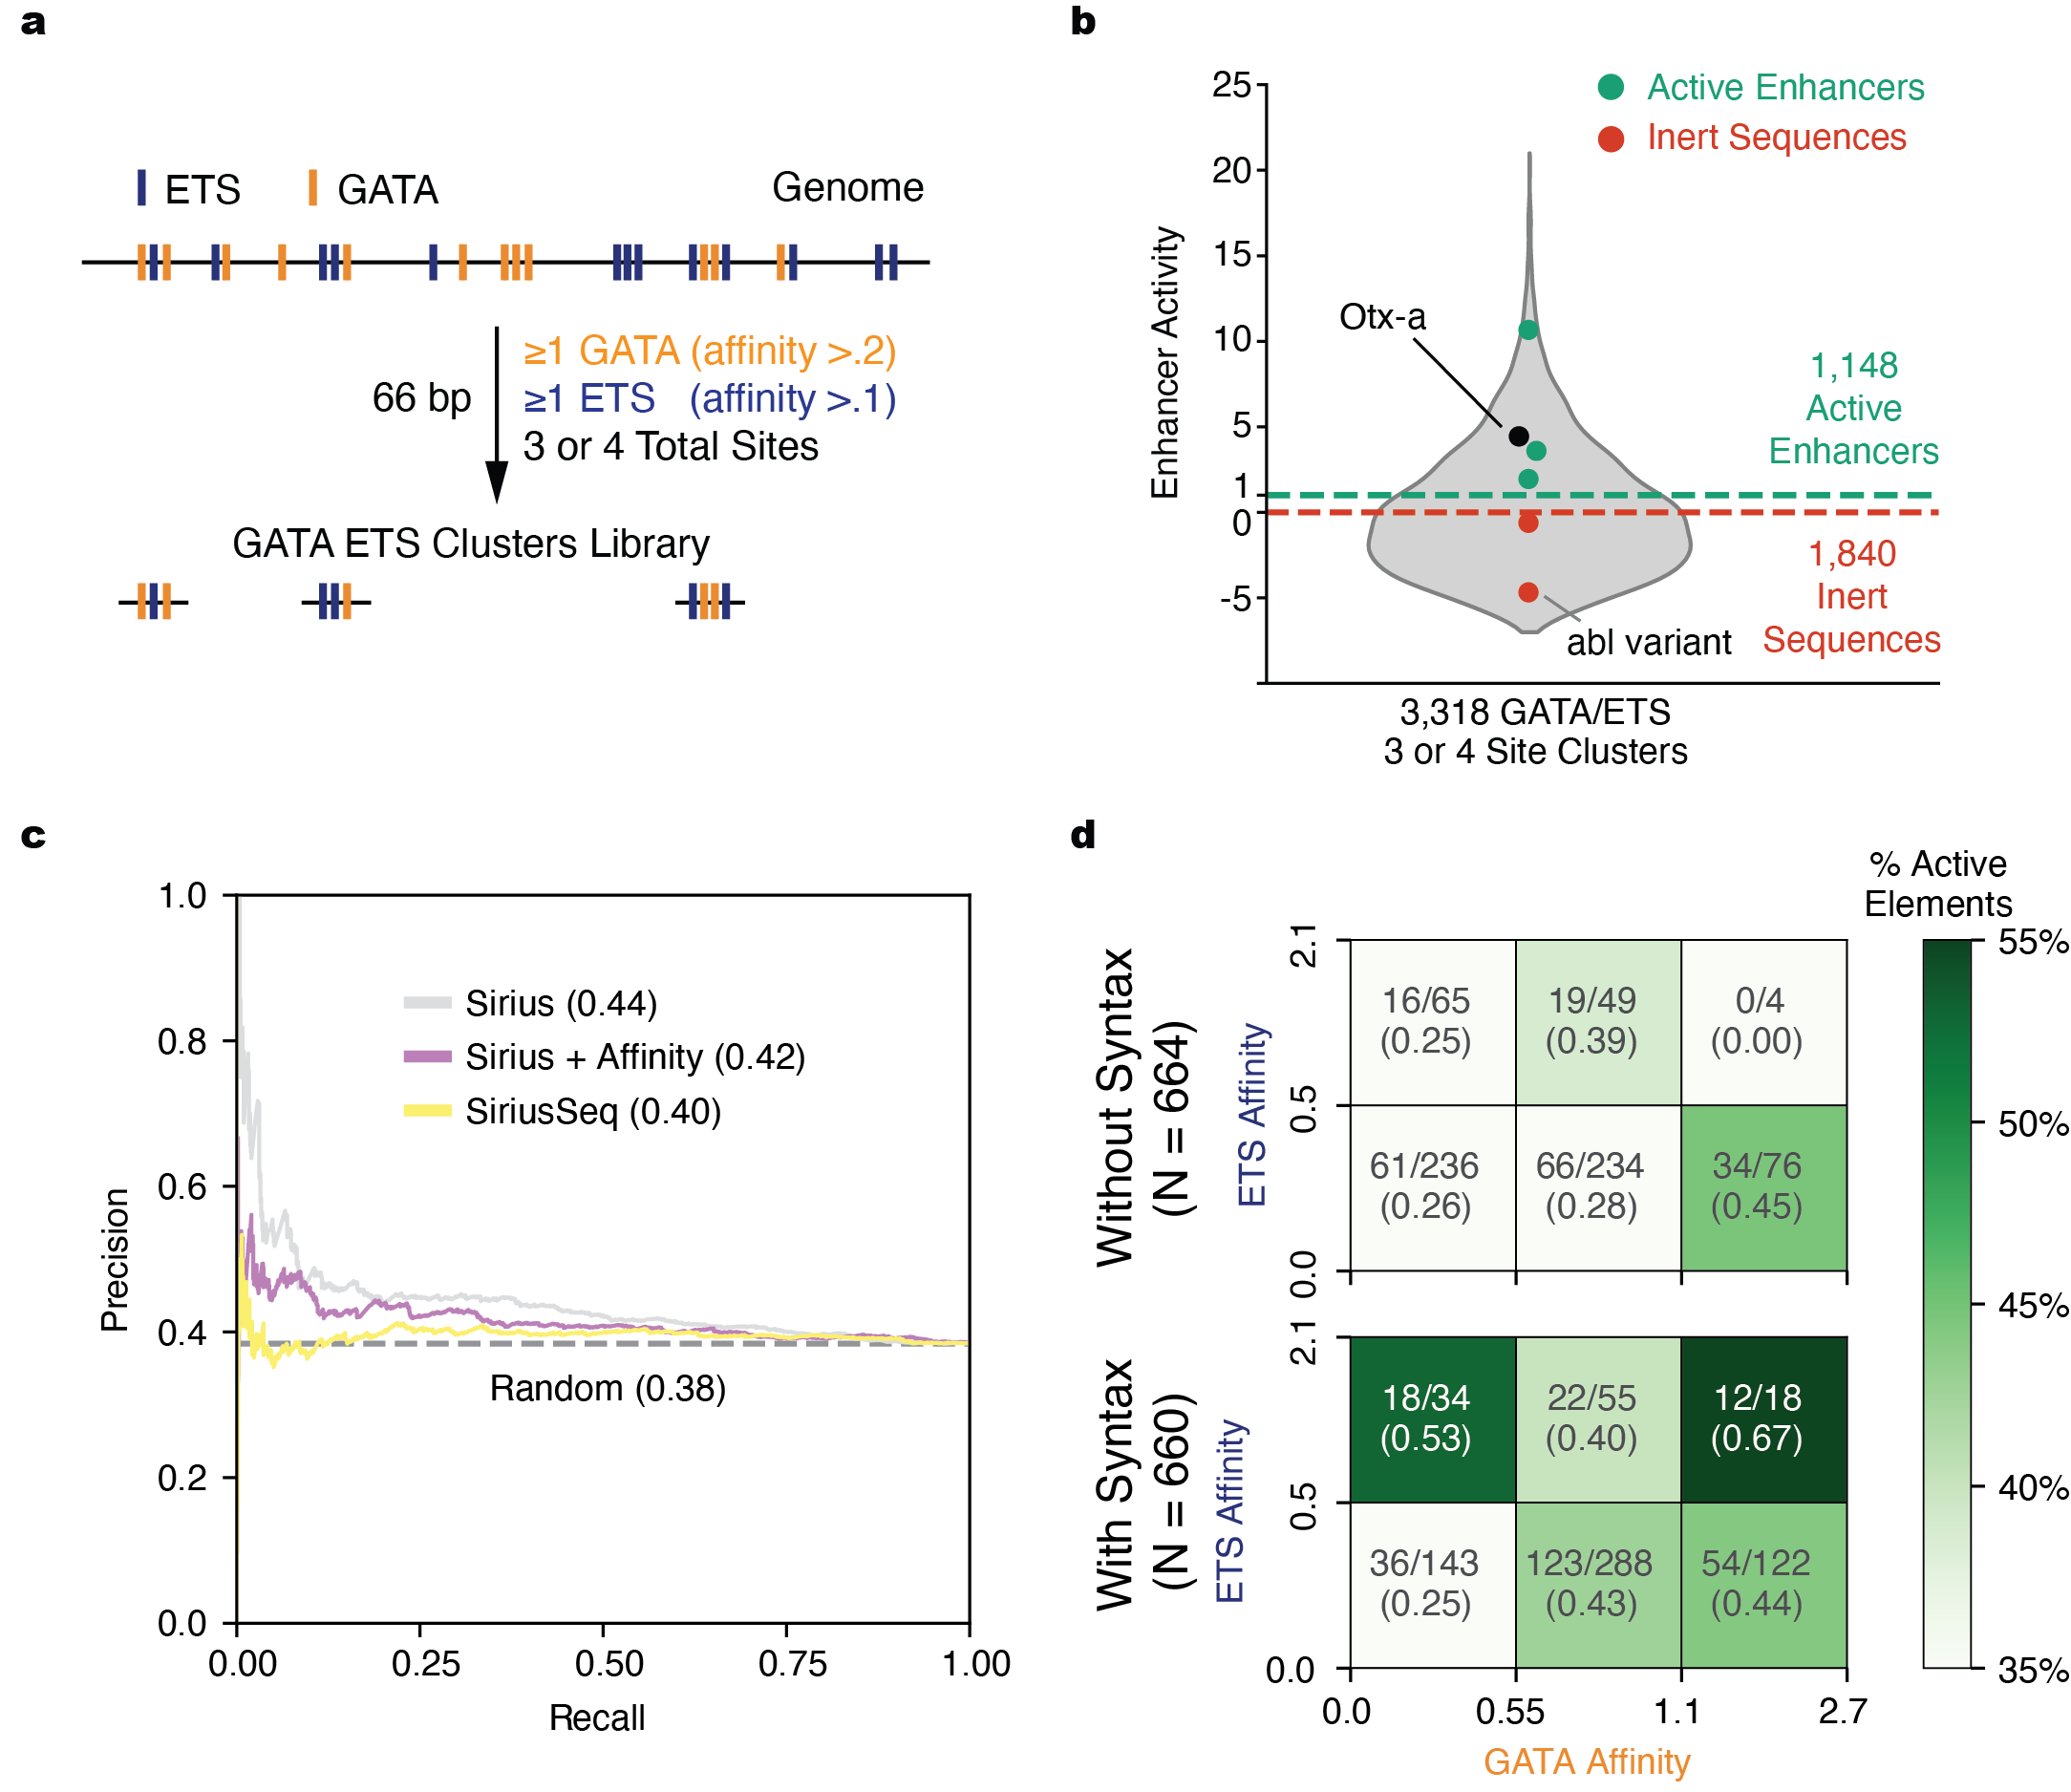
\includegraphics[height=0.7\textheight, keepaspectratio]{2_figures-and-files/Fig5.png}
    \caption[OSL models predict activity of genomic clusters of ETS and GATA sites.]{\textbf{OSL models predict activity of genomic clusters of ETS and GATA sites}.}
    \label{fig:2 Figure 5}
\end{figure}

\clearpage

%%%%%%%%%%%%%%%%%%%%%%%%%%%%%%%%%%%%%%%%%%%%%%%%%%%%%%%%%%%%%%%%%%%%%%%%%%%%%%%%
\section{Discussion}
%%%%%%%%%%%%%%%%%%%%%%%%%%%%%%%%%%%%%%%%%%%%%%%%%%%%%%%%%%%%%%%%%%%%%%%%%%%%%%%%

Years of work combining classical genetics, high-throughput genomic assays, and computational modeling have identified the number, identity, order, orientation, spacing, and affinity of TFBSs as key determinants of enhancer function \cite{Jindal2021-zk}. Yet despite this progress, our understanding of how sequence encodes function remains shallow. Here, we present a novel framework for learning how the sequence of an enhancer encodes function. By combining a deep profile of the grammar of a single enhancer with deep learning, we build an accurate model of enhancer function that successfully guides the design of tissue-specific synthetic enhancers.

The dataset generated in this study represents one of the most exhaustive and well-controlled investigations of enhancer syntax to date. By systematically permuting the order, orientation, and spacing of five experimentally validated TFBS, we created a library of over 900,000 synthetic sequences. Crucially, all elements in the library share the same TFBS identities, numbers, and affinities, allowing us to isolate the functional impact of syntax alone by eliminating confounding variables. When assayed in \textit{Ciona} embryos using MPRA, we found that the majority of TFBS combinations did not drive activity, underscoring the critical role of syntax in function. This result directly supports the idea that the \textit{Otx-a} enhancer is an enhancer that follows a dependency grammar\cite{Jindal2021-zk}, falling in between the enhancesome and billboard models.

A central goal in the study of enhancers is to predict their activity directly from DNA sequence. Most current approaches to this task use deep learning models trained on genomic data \cite{De-Winter2025-nz,Sasse2024-ly}, encoding the nucleotide sequence in an unbiased manner. While these models have proven powerful, disentangling the features they learn (e.g. TFBS identity, affinity, and syntax) and their impact on predictions is not always straightforward. Additionaly, extensive sequence homology in the genome renders them vulnerable to data leakage \cite{De_Boer2024-ic,Rafi2025-er}. Here, we take a complementary approach by representing each sequence in terms of the type, orientation, and position of TFBSs, and demonstrate that syntax alone is sufficient to accurately predict enhancer function in our screen. This approach also enables targeted comparisons of the effect of including specific features, illustrated by our comparisons of models trained on syntax, syntax and affinity, and sequence. Naturally, this approach depends on having prior knowledge of the TFBSs relevant for function and assumes that activity is driven primarily by those sites, which may not hold in more complex or less well-characterized systems. Still, in cases where these conditions are met, syntax-based models offer a powerful and generalizable framework for understanding and predicting enhancer function.

While our model performed well on the synthetic library, it only modestly generalized to the genomic context, as has been previously observed \cite{King2020-hk,Fromel2024-ux}. This suggests an opportunity to refine library designs by introducing greater variability in flanking and linker sequences while maintaining fixed TFBS content, or by using the model itself to design the next iteration of training data \cite{Friedman2023-yh}. Additional improvements may also come from improving the resolution of the synthetic MRPA, both in terms of signal-to-noise ratio and by incorporating tissue-specific readouts. Despite the limitations of the training data, elements with high Sirius scores were consistently enriched for active enhancers across a range of TFBS affinity levels, highlighting that syntax contributes additional predictive signal. These results suggest that syntax is a broadly useful feature for predicting enhancer function, but that it alone is usually insufficient to capture the full complexity of enhancer activity in the genome.

Although neural networks are often viewed as black boxes, model interpretation can help uncover the features they use to make predictions \cite{Novakovsky2022-ft}. In this work, we used a relatively simple marginalization strategy to identify combinations of two and three TFBSs that significantly contribute to enhancer activity and demonstrate that Sirius learns a primarily additive function of these features. This may reflect a billboard model at the level of syntax features rather than individual sites, where only an enhancer with a critical mass of activating syntax features is capable of recruiting a stable transcriptional complex and driving gene expression. Our approach, however, relies on exhaustively enumerating and marginalizing a fixed and tractable number feature combinations, a strategy that may not scale well or generalize to more complex systems. New interpretation methods tailored to syntax models could help uncover non-additive interactions or higher-order rules that are cannot be captured through our margainalization approach. Unsupervised methods in particular, such as clustering learned representations for each sequence, may aid the discovery of latent structure in enhancer grammar and whether that structure operates in distinct states, or along a continuous manifold.

Designing synthetic enhancers with predictable activity has important implications for both basic and translational genomics. Our work complements existing approaches that use large-scale genomic screens or chromatin accessibility data by showing that synthetic screen can be leveraged to design sequences with targeted regulatory activity. Nearly all of our designed enhancers showed tuned expression in the intended direction, and a substantial proportion exhibited MPRA activity consistent with neural-specific enhancers. Initially, we were surprised to find that, despite being trained on bulk data, Sirius could predict function with apparent tissue specificity. One possible explanation for this lies in the primarily additive model Sirius appears to learn. Sirius may be learning that increasing the number of activating syntax features in an enhancer makes it progressively easier to assemble a functional transcriptional complex and that when this assembly becomes too efficient, it will occur even in tissues with lower TF concentrations, leading to broader, less specific activity. This supports the idea that suboptimal syntax is a key determinant of tissue-specific enhancer function\cite{Farley2015-xx,Farley2016-eh}. Still, we assessed enhancer activity using bulk MPRA in this study, and tissue resolved data is ultimately needed to better evaluate Sirius, and to improve the design of tissue-specific enhancers.

Collectively, our study illustrates that enhancer function can be accurately modeled and rationally designed using the syntax of transcription factor binding sites. By systematically dissecting and modeling the grammar of a single developmental enhancer, we demonstrate that the arrangement of a small number of known TFBSs is sufficient to build predictive models, uncover interpretable regulatory rules, and guide the design of synthetic enhancers with tunable, and in some cases, tissue-specific activity. While our framework is grounded in a highly controlled system, its core principles can be extended to other enhancers, cell types, and species, particularly as new experimental tools like single-cell MPRAs \cite{Zhao2023-ql,Lalanne2024-ts} increase the resolution of functional measurements.

%%%%%%%%%%%%%%%%%%%%%%%%%%%%%%%%%%%%%%%%%%%%%%%%%%%%%%%%%%%%%%%%%%%%%%%%%%%%%%%%
\section{Materials and Methods}
%%%%%%%%%%%%%%%%%%%%%%%%%%%%%%%%%%%%%%%%%%%%%%%%%%%%%%%%%%%%%%%%%%%%%%%%%%%%%%%%

\subsection{Ciona}

Adult \textit{Ciona intestinalis} type A (\textit{Ciona robusta}) were obtained from M-Rep (San Diego, CA) and maintained at 18\,\textdegree C in seawater (Reliant Aquariums) under constant illumination. \textit{Ciona} are hermaphrodites, therefore individuals possess a single sex. The age or developmental stage of embryos analyzed is indicated in the main text.

\subsection{Counting embryos}

In \textit{Ciona}, cell identities are well-defined by lineage, allowing each cell to be identified based on visual inspection of nuclear localization signals. GFP expression in individual cells was categorized as weak, moderate, or strong, depending on the exposure time required for clear detection. Fifty embryos were analyzed per biological replicate, and slides were blinded such that the individual performing the counting was unaware of the specific experimental construct being examined. Wild-type (WT) \textit{Otx-a} constructs were included in each experiment as internal references. Statistical significance was determined using Fisher’s exact test.

\subsection{Acquisition of images}

Images of enhancers under comparison were acquired from embryos electroporated on the same day using identical microscope settings. Representative embryos were selected prior to unblinding the slides, based on average expression levels determined during cell counting. Within each figure, images were captured using the same exposure times to facilitate direct comparisons, and all images were cropped identically.

\subsection{Library construction for fluorescence microscopy}

Randomized linker constructs were ordered from IDT with Ns (equal chance of A/C/G/T) in place of linker regions. The enhancer library was transformed using MegaX DHB10 electrocompetent cells with 1,000,000 to 5,000,000 total randomized linker variants.

\subsection{Electroporation for fluorescence microscopy}

All constructs were midiprepped in the same batch with \textit{Otx-a} WT as a control using the NucleoBond Xtra Midi kit (Macherey-Nagel). Dechorionation, in vitro fertilization, and electroporation were performed as described previously\cite{Farley2016-eh}. 70\,\textmu g DNA was resuspended in 100\,\textmu L water and added to 400\,\textmu L of 0.96\,M D-mannitol. Typically for each electroporation, eggs and sperm were collected from 6 adults. Embryos were fixed at the appropriate developmental stage for 15 minutes in 3.7\% formaldehyde. The tissue was then cleared in a series of washes of 0.3\% Triton-X in PBS and then of 0.01\% Triton-X in PBS. Samples were mounted in ProLong Gold Antifade Mountant. GFP images were obtained with an Olympus FV3000, using the 40X objective. All constructs were electroporated in at least two biological replicates.

\subsection{Definitions of \textit{Otx-a} enhancer features}

Transcription factor binding sites (TFBS) for both GATA and ETS consist of a central core of four nucleotides that directly mediate binding through hydrogen bonds, flanked by two nucleotides on each side that modulate binding affinity. For GATA factors, the core sequence is GATA, whereas for ETS factors it is GGAW (where W = A or T). To quantify relative affinities, we used median signal intensities from universal protein-binding microarray (PBM) data obtained for mouse ETS-1\cite{Wei2010-di} and GATA-6\cite{Badis2009-hv} proteins from the UniProbe database (http://thebrain.bwh.harvard.edu/uniprobe/index.php)\cite{Hume2015-xj}. Relative affinity scores for each 8-mer sequence were calculated by dividing the median signal intensity of that sequence by the median intensity of the optimal (consensus) 8-mer. Previous studies indicate that mouse ETS-1 and GATA-6 provide accurate proxies for their \textit{Ciona} homologs, ETS-1 and GATA.a, respectively \cite{Farley2015-xx,Nitta2015-rt,Wei2010-di}. The consensus sites, GAGATAAG (GATA) and CCGGAAGT (ETS), were assigned relative affinity scores of 1.

\subsection{Design of the \textit{Otx-a} scrambled library (OSL)}

The \textit{Otx-a} GATA and ETS scrambled library (OSL) was designed by reorganizing the wild-type (WT) \textit{Otx-a} enhancer with minimal changes to sequence content. To eliminate an unintended ETS core (GGAW) in Linker 1 of the WT sequence, the first three bases of this linker were removed, resulting in a 66\,bp construct. In Linker 4, a TTC motif was modified (TGTTC~$\rightarrow$~TGCTC) to prevent formation of a de novo ETS core (TTCC) when positioned adjacent to C-starting motifs, such as reverse-strand GATA sites (e.g., CATC). These modifications did not alter \textit{Otx-a} expression. The WT sequence was segmented into transcription factor binding sites (TFBSs) and linkers, and every possible permutation of the structure Linker–TFBS–Linker–TFBS–Linker–TFBS–Linker–TFBS was generated. This yielded $2^5 \times 5! \times 5! = 460{,}800$ OSL variants. We additionally generated another 460,800 variants with point mutations to sites known to ablate binding to each GATA (GATA$>$AATA)\cite{Bertrand2003-su} and ETS (GGAW$>$GCAW)\cite{Woznica2012-jd,Schachterle2012-kq}. In total, there are 921,600 sequences in the GATA and ETS OSL. The oligonucleotide library was synthesized by Twist Bioscience.

\subsection{Library cloning}

Both the GATA and ETS OSL and the genomic clusters library were cloned with the following steps. The enhancer variants were ordered from Agilent Technologies with adapters containing BseRI sites. This was cloned into the custom-designed SEL-Seq (Synthetic Enhancer Library-Sequencing) vector using type II restriction enzyme BseRI\cite{Farley2016-eh}. After cloning, the library was transformed into MegaX DH10B electrocompetent cells, and the culture was grown up until an OD of 1 was reached. DNA was extracted using the Macherey-Nagel Nucleobond Xtra Midi kit. A 30\,bp barcode with adapters containing Esp3I sites was cloned into this library using type II restriction enzyme Esp3I. The library was transformed into MegaX DHB10 electrocompetent cells and grown up until an OD of 1 was reached. The DNA library was extracted from the bacteria using the Macherey-Nagel Nucleobond Xtra Midi kit. The GATA and ETS OSL members contain 54 unique barcodes per enhancer. The GATA and ETS genomic clusters library members contain 12 unique barcodes per enhancer.

\subsection{Enhancer to barcode assignment}

To determine which enhancer was associated with which barcode tag, we removed the intervening sequence containing promoter and GFP by restriction digest with XbaI and SacI and re-ligated the remaining vector to get the enhancer and barcode in close proximity. We amplified the region of interest with 10 cycles of PCR, and size-selected the PCR product using Agencourt AMPure XP beads. We ran the purified sample on a bioanalyzer to check the product was the correct size. The OSL and the GATA ETS genomic elements library were sequenced using NovaSeq S4 PE150 mode (Illumina).

\subsection{Enhancer to barcode dictionary analysis}

Raw sequencing data was first deduplicated to get a file with unique reads and associated read counts. The location of the barcode and enhancer in the read is known based on the vector design. For each unique read, we searched for the enhancer in the expected location $-5$ to $+1$\,bp. If the sequence at the enhancer location is a perfect match to a sequence we ordered, then we extract the enhancer from the read and the first 25\,bp as the barcode.

\subsection{Massively-parallel reporter assay (MPRA)}

Each library was electroporated into $\sim$500,000 fertilized eggs. Embryos were developed until 5\,hrs 15\,min at 22\,\textdegree C (gastrula stage). Embryos were then put into TRIzol, and RNA was extracted following the manufacturer’s instructions (TURBO DNA-free Kit, Invitrogen). The RNA was DNase treated using Turbo DNase I from Ambion following standard instructions. Poly-A selection was used to obtain only mRNA using poly-A magnetic beads as per instructions (Dynabeads mRNA Purification Kit, Life Technologies). The mRNA was used in an RT reaction that specifically selected for the barcoded mRNA (Transcriptor High Fidelity cDNA Synthesis Kit, Roche). The RT product was PCR amplified and size-selected using Agencourt AMPure XP beads (Beckman Coulter), then checked for quality and size on the 2100 Bioanalyzer (Agilent) and sent for sequencing on the NovaSeq S4 PE100 mode (Illumina). At least three biological replicates were sequenced for both the OSL and the GATA and ETS genomic clusters library.

The DNA was extracted by mixing the phenol-chloroform and interphase of TRIzol extraction with 500\,\textmu L of Back Extraction Buffer (4\,M guanidine thiocyanate, 50\,mM sodium citrate, and 1\,M Tris-base). DNA was treated with RNase A (Thermo Fisher). DNA was cleaned up with Phenol:Chloroform:Isoamyl alcohol (25:24:1) (Life Technologies). The DNA was PCR amplified and size-selected using Agencourt AMPure XP beads (Beckman Coulter), then checked for quality and size on the 2100 Bioanalyzer (Agilent) before sequencing on the NovaSeq S4 PE100 mode (Illumina). At least three biological replicates were sequenced for OSL and the GATA and ETS genomic elements library.

\subsection{Quantification and classification of enhancer activity}

Barcodes were extracted as the first 25 bases of each sequenced read. Read counts per barcode were summed and normalized to reads per million (RPM). For each replicate, RNA and DNA reads were aggregated separately by summing RPMs across all barcodes assigned to each enhancer, based on a predefined barcode-enhancer mapping. Enhancer activity was defined as the ratio of summed RNA RPM to summed DNA RPM. Enhancers with activity $< 0.5$ in any replicate were excluded from analysis. Activity scores from remaining replicates were summed and log$_2$-transformed to produce a single activity value per enhancer \cite{Ashuach2019-qp}. A subset of elements ($n = 23$) was selected for validation by fluorescence microscopy, and activity thresholds were established by identifying cut-offs that best separated validated inert and active enhancers. These thresholds corresponded to the 45th and 85th percentiles of the distribution. Activity values were linearly rescaled such that the 45th percentile equaled 0 and the 85th percentile equaled 1. Elements with rescaled activity $< 0$ were classified as inert sequences, $> 1$ as active enhancers, and those between $0$ and $1$ as weak enhancers. Only inert and active elements were used for downstream analysis.

\subsection{Syntax encoding}

We evaluated multiple strategies for encoding DNA sequence as input to models of enhancer function, broadly categorized into syntax-based and sequence-based encodings. For syntax encodings, we developed a flexible representation that balances prior knowledge of transcription factor binding sites (TFBSs) with the capacity of neural networks to learn higher-order combinatorial rules. This approach mitigates overfitting to spurious sequence features that may be correlated with TFBS presence due to the structured design of the dataset. Sequences were encoded across four channels corresponding to GATA and ETS sites in both forward and reverse orientations; a value of 1 was assigned at positions where a given TFBS occurred (GATA = “GATA”, ETS = “GGAW”). This encoding enables unbiased learning of positional, type, and orientation relationships between sites. 

We also experimented with adding affinity to this encoding by modifying the four original channels to include separate channels for each affinity of the binding site (G1 = 0.85, G2 = 0.32, G3 = 0.45, E1 = 0.58, E2 = 0.39). The resulting input has 10 channels for the forward and reverse orientation of each site. Finally, we implemented a shallow machine learning model using hand-crafted features per binding site. This includes ETS and GATA affinity scores, binary orientation indicators, and scaled linker lengths and is limited to sequences containing exactly five binding sites (\textbf{Supplementary Table 3}).

\subsection{Sirius training, validation, and benchmarking}

\subsubsection{Training, validation and test splits}

Many elements in the OSL library have distinct linear DNA sequences but the same syntax (the functional organization of binding sites). Each of these elements with the same syntax differ only by the linkers and flanking nucleotides of the cores at each site, modulating their affinities. Across the 460,800 elements, there are 103,680 unique syntaxes. We took 90\% of syntaxes (93,312) to construct a training set, corresponding to 414,228 sequences. From this set, 46,756 active enhancers were selected as positives based on two criteria: (1) the WT sequence was classified as active, and (2) the corresponding ablated version was classified as inactive or undetected. We call these sequences GATA and ETS dependent sequences. A matched set of 46,756 negative sequences was drawn from the remaining training syntaxes with the lowest activity scores. For each model type, we performed ten-fold cross-validation over the training set, with 84,240 syntaxes used for model fitting and the remainder reserved for hyperparameter optimization and early stopping. Model selection was based on the validation loss. The test set consisted of the remaining 10\% of syntaxes (10,368), representing 46,572 sequences. Positive and negative examples in the test set were defined using the same criteria as the training set, except that all inert sequences were retained to reflect the true class distribution in the experiment. Model performance was evaluated on held-out data using auPRC and auROC.

\subsubsection{Syntax model benchmarking}

We benchmarked several classes of neural network architectures trained on the syntax encoding. Each model was trained on a single fold of the training split for a maximum of 25 epochs. Parameters of each model were updated via backpropagation of the gradient from a binary cross entropy loss function with the Adam optimizer\cite{Kingma2014-kn}. The model with the best auPRC on the validation examples for that fold was used for all downstream performance comparisons and experiments. Neural network optimization was performed using PyTorch (v2.1.0) on NVIDIA A30 GPUs.

Shallow models benchmarking of syntax encodings consisted of logistic regression, random forests, and gradient boosted machines, each using the same set of hand-crafted features. Hyperparameters for each shallow model type were optimized via a grid search using scikit-learn (v1.3.0). We called the best performing model, a neural network architecture based on ResidualBind\cite{Koo2021-ly} with dilated-residual convolutions, Sirius. All downstream analysis and sequence design was performed using the model trained on the first fold.

\subsubsection{Alternative Sirius training strategies}

\paragraph{Training a classifier on all active enhancers}

We also benchmarked the above training paradigm for Sirius against two other strategies. In the first, we did not force sequences in the training set to have an ablated counterpart classified as inactive or undetected. In this training set, we have 72,834 positive sequences and a matched set of 72,834 negative sequences drawn from the remaining training syntaxes with the lowest activity scores. We term this the models trained on this set as “Sirius Active Enhancers” and the model trained on the previously described set as the “Sirius GATA/ETS Dependent” model.

\paragraph{Training a regression model to predict enhancer activity levels}

The second alternative strategy we employed was to train a model to predict the enhancer activity levels directly in a regression task rather than binarize them. In this setting, we do not remove weak enhancers, and instead include all 393,554 sequences detected in the library. We use the same training and test splitting and keep all aspects of model training the same, except for using mean squared error as the loss function during training, and validation Pearson correlation coefficient (PCC) for early stopping and benchmarking. We call models trained in this fashion “Sirius Regression” models. 

Sirius Regression models produce a continuous valued output that can be naturally compared to enhancer activity for evaluation. Classification models by definition produce a log odds (logit) as an output which is transformed into a probability using the sigmoid function. For evaluating Sirius on activity level predictions we calculated the PCC between the logits and the MPRA activity levels. For simplicity, we refer to the logits as “Model Predictions” throughout the main text and figures and the sigmoid transformed probabilities as “Model Probabilities.”

\subsection{Sequence model evaluation}

\subsubsection{Training sequence models}

We also benchmarked Sirius\textquotesingle s performance against two models that take in a more unbiased representation of the linear DNA sequence as input. We evaluated the same dilated-residual CNN architecture operating on one-hot encoded linear DNA sequence (A = [1, 0, 0, 0], C = [0, 1, 0, 0], ..), which we call SiriusSeq, and support vector machines on gapped k-mers (gkmSVMs) \cite{Ghandi2014-hn}. SiriusSeq was trained in the same manner as Sirius. We used the default parameters of the \texttt{ls-gksvm} package for training all gkmSVM as changing these parameters did not significantly affect performance.

\subsubsection{Randomization of features and test set performance}

We evaluated the most important features learned by SiriusSeq by comparing the test set auROC and auPRC on unperturbed sequences to the following versions of the test set sequences:

\begin{itemize}
    \item \textbf{Flanks} – Randomization of the two nucleotides on either side of the four core base pairs of each site. Four total nucleotides are randomized per site, 20 per sequence.
    \item \textbf{Linkers} – Randomization of all nucleotides \textit{not} contained in the binding site cores or the two flanking nucleotides on either side of the core. 27 total nucleotides are randomized per sequence.
    \item \textbf{Cores} – Randomization of the four core base pairs of each site. Four total nucleotides are randomized per site, 20 per sequence.
    \item \textbf{TFBS} – Randomization of the four core base pairs of each site \textit{and} the two nucleotides on either side of the core. Eight total nucleotides are randomized per site, 39 per sequence.
\end{itemize}

Each randomization is carried out by independently selecting an ‘A’, ‘C’, ‘G’ or ‘T’ at each position to be randomized with uniform 0.25 probability.

\subsubsection{De novo motif discovery with TF modisco}

We took all 52,139 GATA and ETS dependent enhancers and a matched set of 52,139 negative sequences from the remaining sequences with the lowest activity scores and computed nucleotide resolution attributions for each sequence using the DeepLiftShap implementation in tangermeme (v0.4.2) on SiriusSeq. We passed these attributions to the TF-modisco algorithm as implemented in the modisco-lite package (v2.2.1) using max\_seqlets\_per\_metacluster=1\_000\_000, sliding\_window\_size=15, flank\_size=5, target\_seqlet\_fdr=0.2.

\subsection{Syntax feature discovery}

\subsubsection{Organizational feature definition}

Organizational features are encoded using order, orientation and spacing of GATA and ETS binding sites. We exhaustively enumerated all possible orders, orientations and spacings for all pairs of binding sites (GATA-ETS, GATA-GATA, ETS-ETS), called 2-site organizational features, and all possible triplets of binding sites (GATA-GATA-GATA, GATA-GATA-ETS, etc.), called 3-site organizational features. Since each element has a total of 5-sites, this means that there are a total of 10 possible 2-site (5 choose 2) and 10 possible 3-site (5 choose 3) features in each element. Repeating this feature generation across all 460,800 elements gives a total of 9,022 unique organizational features.

\subsubsection{Organizational feature marginalization with Sirius}

We first made predictions for all 460{,}800 OSL elements using Sirius. For each of the 9{,}022, we split the predictions into two groups: those that were made on sequences that contained the feature and those that did not. We then ran a Mann--Whitney U-test comparing the two distributions to assess statistical significance, and corrected the 9{,}022 $p$-values using the Benjamini--Hochberg method. We calculated the relative mean odds ratio and applied a log base 2 transformation to quantify the effect of each organizational feature. To do so, we calculated the mean of the logits for each group (feature vs.\ no feature), exponentiated each to obtain a mean odds for each group, calculated the relative odds as the ratio of feature odds to no-feature odds, and then applied a log base 2 transformation. We used cut-offs of corrected $p$-value $< 0.001$ and absolute log-ratio $> 1$ to define syntax features (significant organizational features). When negative, this value represents a decrease in predicted odds for sequences containing the feature compared to those that do not, which we call an inactivating syntax feature. When positive, this represents an increase in predicted odds, which we call an activating syntax feature.

\subsubsection{Organizational feature analysis}

\paragraph{Positional specificity analysis}

To determine if organizational features exhibited any positional relationship with function, we slid each organizational feature across every possible position of a background sequence and made predictions with Sirius. Background sequences were composed with all N’s to isolate the effects of each feature. This produced a variable number of predictions for each organizational feature that was dependent on the size of the feature. For each set of predictions, we calculated a normalized center of mass across all possible positions by first calculating a raw center of mass score: \(\texttt{com\_raw = np.sum(pos\_vals * prob)}\) and then min-max scaling it: \(\texttt{com\_norm = (com\_raw - pos\_vals.min()) / (pos\_vals.max() - pos\_vals.min())}\).

\paragraph{Single flip analysis}

To test whether single syntax changes can alter the effect of an organizational feature, we examined all 3-site features and identified pairs in which one syntax variant had a $\log_2$ relative mean odds $> 0$ while its counterpart had $< 0$.

\paragraph{AdditiveFeatures model}

To investigate the independent and additive contributions of organizational features, we devised a simple model using all 9,022 organizational features. For each sequence, we sum the effect sizes over all organizational features the sequence contains. This produces a continuous value for each sequence that can be compared to the true labels in the same way Sirius predictions can.

\subsection{Sirius-guided enhancer design}

\subsubsection{Binning sequences by tissue specificity}

To systematically assess the level to which Sirius predictions were tissue-specific, we refined our sequence classifications for each element of the OSL library to include Inert Sequences, Neural Enhancers, or Ectopic Enhancers based on the following criteria:

\begin{itemize}
  \item \textbf{Inert Sequences:} Syntax score \textless 5; 0 active enhancer siblings, \(\geq\) 7 inert sequence siblings; MPRA activity score \(\leq\) 0
  \item \textbf{Neural Enhancers:} Syntax score 18--22; 4 or 5 active enhancer siblings, 2 or 3 inert sequence siblings; MPRA score 1--1.5 (Otx-a WT = 1.2)
  \item \textbf{Ectopic Enhancers:} Syntax score \(\geq\) 30; 7 active enhancer siblings, 0 inert sequence siblings; MPRA activity score \(\geq\) 2
\end{itemize}

We used previously calculated syntax scores for each OSL member and defined siblings as sequences with a fixed order, orientation, and spacing of sites. See \cite{Solvason2024-gi} for more details.

\subsubsection{STARS design}

\paragraph{Syntax edits}

We defined four types of possible edits for design:
\begin{itemize}
  \item \textbf{Ablate:} Remove a single binding site (flip the 0 to 1 for that binding site in the syntax encoding)
  \item \textbf{Flip:} Change the orientation of a single binding site (shift the 1 in a channel to the other channel of the other orientation for the same binding site: 0\(\leftrightarrow\)2, 1\(\leftrightarrow\)3)
  \item \textbf{Switch:} Change the type of a binding site but keep the orientation the same (0\(\leftrightarrow\)1, 2\(\leftrightarrow\)3)
  \item \textbf{De novo:} For each possible position, add each possible binding site (flip the 1 to 0 for that position and binding site). We forced the de novo site to have a gap of 7\,nt from any other existing site or sequence edge.
\end{itemize}

\paragraph{Iterative design}

We implemented an iterative design procedure to generate synthetic enhancers using the Sirius model. At each iteration, one of the four edit types was randomly selected to ensure balanced sampling. All possible single-site edits of that type were enumerated to generate a candidate pool. Each candidate was scored using a Sirius-derived objective function, and the optimal candidate was selected as the new starting syntax. This process was repeated for a fixed number of iterations.

\paragraph{STARS design parameters}

To design STARS (Syntax-derived, Tissue-specific, Active Regulatory Sequences), we used an objective function that minimized the absolute difference between Sirius predictions and a target value of 1.52, corresponding to the median activity of neural enhancers (\textbf{Supplementary Figure~\ref{fig:2 supplementary_10c}}). Design runs proceeded for 25 iterations and were constrained to:
\begin{itemize}
  \item contain 4--6 binding sites,
  \item avoid duplicate syntaxes within a run.
\end{itemize}

To select sequences for validation, we filtered for exactly five binding sites, at least two ETS and two GATA sites, and predicted score within 0.2 of the target. We excluded any sequences overlapping the OSL library.

Two classes of STARS were designed:
\begin{itemize}
  \item \textbf{Activated:} 14 inert syntaxes from the OSL library.
  \item \textbf{Tuned:} Two ectopic syntaxes (R12A1/2 and R10B1/3), each used to generate five designs.
\end{itemize}

\subsubsection{STARS bulk MPRA library design}

To validate STARS activity, we designed a bulk MPRA library. For each of 24 STARS (14 activated, 10 tuned), eight variants were generated by modifying the binding site context, yielding 192 synthetic sequences.

\paragraph{Flanking sequence selection (affinity placement)}

Each syntax was tested under four flanking sequence contexts:
\begin{itemize}
  \item \textbf{Random placement:} Affinity classes (e.g., G1, G2, G3) were randomly assigned.
  \item \textbf{Sirius + Affinity-guided placement:} All combinations scored using the Sirius + Affinity model, selecting configurations closest to neural enhancer median.
\end{itemize}

Flanks preserved affinity within \(\pm0.03\) of the original \textit{Otx-a} WT site and avoided: (i) new TFBSs, (ii) restriction sites, (iii) adapter junction motifs.

\paragraph{Linker selection}

Linkers were sampled from two inert backbones to avoid introducing new motifs or restriction sites.

\paragraph{Control sequences}

Matched ablated versions of each STARS were generated by mutating core bases (e.g., GATA\(\rightarrow\)AATA). Ablated variants were screened to avoid introducing new motifs or restriction sites. 37 validated controls from the OSL library were also included.

\paragraph{Final library composition}

Each of the two sub-libraries (targeting 1000 barcodes) included:
\begin{itemize}
  \item 96 designed STARS (7 activated + 5 tuned) \(\times\) 8 variants
  \item 96 ablated counterparts
  \item 37 control sequences
\end{itemize}

Each enhancer had 5 barcodes, for 1,145 total constructs per sub-library. Libraries were synthesized by Twist Biosciences.

\subsubsection{STARS bulk MPRA analysis}

Barcodes (first 25\,bp of each read) were normalized to reads per million (RPM). Barcodes with DNA or RNA RPM \textless 15 were excluded. RNA:DNA ratios were calculated per barcode, aggregated by median across barcodes per enhancer, and log$_2$-transformed.

To assess label accuracy, activity thresholds were calibrated against 37 previously validated elements. Enhancers were classified as:
\begin{itemize}
  \item \textbf{Inert:} Rescaled activity \textless 0
  \item \textbf{Neural:} 0 \(\leq\) activity \(\leq\) 1
  \item \textbf{Ectopic:} Activity \textgreater 1
\end{itemize}

\subsection{Genomic MPRA library design}

We extracted all 66\,bp tiles that included 3 or 4 non-overlapping binding sites, with at least one GATA (matching "GATA" with affinity \(\geq 0.2\)) and one ETS (matching "GGAW" with affinity \(\geq 0.1\)) site. This resulted in a library of 3,312 sequences. The oligo library was synthesized by Twist Biosciences.

\subsubsection{Genomic MPRA analysis}

\paragraph{Enhancer activity calculation}

Barcodes were extracted as the first 25 bases of each read. Read counts were normalized to reads per million (RPM), and barcodes with DNA RPM \textless{} 0.05 were excluded. Enhancers with fewer than five DNA-detected barcodes were removed. Barcode RPMs were aggregated by enhancer, and RNA:DNA ratios were averaged across replicates. Replicates with enhancer activity \textless{} 0.5 were considered undetected and excluded. Sequence-level scores were calculated by summing remaining replicate activities, log$_2$ transformed, and rescaled such that the 55th percentile equals 0 and the 65th percentile equals 1. Elements with rescaled activity \textless{} 0 were considered inert; those \textgreater{} 1 were active enhancers.

\subsubsection{Models trained on genomic elements}

Only binding sites with affinity \textgreater{} 0.1 (ETS) or \textgreater{} 0.2 (GATA) were considered. Of the 3,318 elements tested, 3,170 had unique syntaxes. 90\% of syntaxes (2,853) were used for training (2,986 sequences), including 1,033 active enhancers and a matched set of 1,033 negatives. Three-fold cross-validation was performed, using 1,382 syntaxes for training and the remainder for validation and early stopping. The held-out test set consisted of the remaining 10\% of syntaxes (317), totaling 326 sequences. Positive and negative test labels were defined as in training, but all inert sequences were retained. Model performance was evaluated using auPRC, auROC, and Pearson correlation (logits vs. enhancer activity). To assess generalization, OSL-trained models (unexposed to genomic sequences) were evaluated on all 3,318 elements. Enhancers were binarized and auPRC computed.

All models used a dilated-residual CNN architecture, trained on one fold for up to 100 epochs. Binary cross entropy loss was optimized using Adam\cite{Kingma2014-kn} (learning rate = 0.0001), batch size 32, and early stopping based on validation loss. Fine-tuning initialized weights from OSL models. Training was performed in PyTorch (v2.1.0) on NVIDIA A30 GPUs.

\subsubsection{mESC analysis}

Synthetic and genomic MPRA datasets were obtained from \cite{King2020-hk}. For the synthetic MPRA, models were trained on log$_2$-transformed normalized activity scores. Data were split into training and test sets per the original study. Syntax encodings used consensus motifs for Sox2 ("GCTCATTGTTTC"), Pou5f1 ("GGGATGCTAATC"), Esrrb ("GTTCAAGGTCAC"), and Klf4 ("GGGGTGGGGCCG"). Performance was measured by \(R^2\), Pearson correlation, and Spearman's \(\rho\). Training used the same architecture, mean squared error loss, Adam optimizer (learning rate = 0.001), batch size 16, and early stopping.

For the genomic MPRA, enhancer activity was binarized by selecting the top and bottom 25\% of gWT elements (101 positives, 101 negatives). Models were trained using the same architecture. Syntax + affinity encodings used FIMO motif matches (p-value \textless{} 0.01) with PWMs from JASPAR\cite{Castro-Mondragon2022-kx}.

\subsubsection{Statistical methods}

Mann-Whitney U tests\cite{Mann1947-dw} were used to compare performance distributions, with Benjamini-Hochberg correction\cite{Benjamini1995-da}. TomTom alignment significance was based on\cite{Gupta2007-zw}, and matches with q-value \(\leq 0.05\) were deemed significant.

%%%%%%%%%%%%%%%%%%%%%%%%%%%%%%%%%%%%%%%%%%%%%%%%%%%%%%%%%%%%%%%%%%%%%%%%%%%%%%%%
\section{Data availability}
%%%%%%%%%%%%%%%%%%%%%%%%%%%%%%%%%%%%%%%%%%%%%%%%%%%%%%%%%%%%%%%%%%%%%%%%%%%%%%%%

All data supporting the findings of this study are available within the paper and its Supplementary Information. mESC MPRA data analysed in this paper were downloaded from Supplementary Information in \cite{King2020-hk}.

%%%%%%%%%%%%%%%%%%%%%%%%%%%%%%%%%%%%%%%%%%%%%%%%%%%%%%%%%%%%%%%%%%%%%%%%%%%%%%%%
\section{Code availability}
%%%%%%%%%%%%%%%%%%%%%%%%%%%%%%%%%%%%%%%%%%%%%%%%%%%%%%%%%%%%%%%%%%%%%%%%%%%%%%%%

Code for dataset construction, model training, and evaluation were performed with EUGENe v0.0.8 \cite{Klie2023-yr} and \url{https://github.com/Enhancer-Grammar/SyntaxNN/tree/main}. Code used for data analysis and generating figures can be found at \url{https://github.com/Enhancer-Grammar/otxa-enhancer-grammar}.

%%%%%%%%%%%%%%%%%%%%%%%%%%%%%%%%%%%%%%%%%%%%%%%%%%%%%%%%%%%%%%%%%%%%%%%%%%%%%%%%
\section{Acknowledgements}
%%%%%%%%%%%%%%%%%%%%%%%%%%%%%%%%%%%%%%%%%%%%%%%%%%%%%%%%%%%%%%%%%%%%%%%%%%%%%%%%

We thank all members of the Carter and Farley labs for many helpful discussions. This work was supported by the National Institutes of Health [grant number 1U01HG012059]; infrastructure was funded by the National Institutes of Health [grant number 2P41GM103504-11]. E.K.F and J.J.S were supported by the National Institutes of Health [grant number DP2HG010013]. H.C. is supported by the Canadian Institute for Advanced Research [award number FL-000655].

%%%%%%%%%%%%%%%%%%%%%%%%%%%%%%%%%%%%%%%%%%%%%%%%%%%%%%%%%%%%%%%%%%%%%%%%%%%%%%%%
\section{Author Contributions Statement}
%%%%%%%%%%%%%%%%%%%%%%%%%%%%%%%%%%%%%%%%%%%%%%%%%%%%%%%%%%%%%%%%%%%%%%%%%%%%%%%%

A.K., J.J.S., E.K.F. and H.C. designed the study. J.J.S. performed the OSL MPRA design and analysis. A.K. trained, evaluated and interpreted all models, implemented the synthetic enhancer design, and designed the STARS MPRA. K.T. performed the STARS MPRA. S.K.J. performed the STARS MPRA analysis. F.L. performed the fluorescence microscopy validation. J.H. performed the mESC MPRA analysis. A.K. wrote the manuscript. H.C. and E.K.F. supervised the work.

%%%%%%%%%%%%%%%%%%%%%%%%%%%%%%%%%%%%%%%%%%%%%%%%%%%%%%%%%%%%%%%%%%%%%%%%%%%%%%%%
\section{Competing Interests Statement}
%%%%%%%%%%%%%%%%%%%%%%%%%%%%%%%%%%%%%%%%%%%%%%%%%%%%%%%%%%%%%%%%%%%%%%%%%%%%%%%%

The authors declare no competing interests.

%%%%%%%%%%%%%%%%%%%%%%%%%%%%%%%%%%%%%%%%%%%%%%%%%%%%%%%%%%%%%%%%%%%%%%%%%%%%%%%%
\section{Inclusion and Ethics Statement}
%%%%%%%%%%%%%%%%%%%%%%%%%%%%%%%%%%%%%%%%%%%%%%%%%%%%%%%%%%%%%%%%%%%%%%%%%%%%%%%%

All research was conducted and is relevant locally.
